%!TEX root = ../thesis.tex
%*******************************************************************************
%*********************************** First Chapter *****************************
%*******************************************************************************

\chapter{Background}  %Title of the First Chapter


\section[Research Hypothesis]{Research Hypothesis}

This chapter presents an introduction to neuromorphic engineering and its fundamental concepts.  These concepts are categorised into different groups and analysed with more detail in relation to the overall study. In the context of this thesis, each topic's fundamental ideas are concisely explained. 

\section[Device Material Characteristics]{Device Material Characteristics}

Extensive research has been conducted in device physics and material science to explore innovative materials and techniques for memories and prolonged retention objectives \cite{indiveri2021introducing}.  The term "neuromorphic" was created by researchers to describe new technologies and systems that, in addition to being essential for the construction of massive AI computer networks, exhibit certain behaviours that can be compared to those of real synapses \cite{di2009circuit}. \\

\noindent Soon after, the notion of using these novel nanoscale components as "memristors" gained popularity, with the underlying notion being that they could be utilised to produce synapses in deep neural networks and sustain their synaptic weights locally \cite{jo2010nanoscale}.  The hardware and technology described could enable neural networks to perform "in-memory computing" and exhibit advanced non-linear properties, mimicking the physics of biological synapses \cite{saighi2015plasticity}. \\

\noindent The research in this field aims to develop various types of volatile and non-volatile memristive electronics. Additionally, spike or pulse-based control systems are being created to elicit biologically realistic learning behaviours in memristive cross-bar arrays.  The challenging task is to find the perfect artificial synapse, which requires investigation into different materials, tools, and techniques.

\subsection[Theoretical Foundations]{Theoretical Foundations}

The presence of symmetry in nature, which is believed to arise from a common origin, is remarkable.  However, the traditional electromagnetic passive circuit components of resistor, capacitor, and inductor are inadequate for describing the characteristics connected by the symmetry of circuit theory. Leon Chua addressed this issue by introducing the concept of a memristor in 1971 \cite{chua1971memristor}, which couples flux linkage and charge as a circuit device. However, proof of resistive switching in the memristor model was not established until 2008 \cite{strukov2008missing}. \\

\begin{figure}[htbp!] 
\centering    
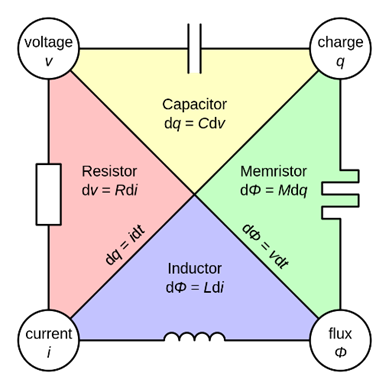
\includegraphics[width=0.5\textwidth]{Chapter1/Figs/1a.png}
\caption[Conceptual symmetries of resistor, capacitor, inductor, and memristor]{Conceptual symmetries of resistor, capacitor, inductor, and memristor \cite{du2017metal}. These four fundamental variables in circuit theory are depicted with their relationships. Each variable can be related to another via either a passive component or a well-known equation.}
\label{fig:1a}
\end{figure}

\noindent There are three fundamental circuit elements and four essential circuit variables in basic electrical circuit theory.  It is evident that one component is absent to achieve symmetry. This device ought to function in such a way that charge and magnetic flux are interconnected, as illustrated in Figure \ref{fig:1a}. The link between the mathematical memristive model and a two-terminal resistive switching device is pivotal in this instance. \\

\noindent The concept of memristance differs from that of resistance in that it is dependent on charge, rather than being a constant value.  As current is the amount of charge flowing per unit time, we can express it as $q = \int_{-\infty}^{t_0} i(t)dt$, where charge is the sum of current at a given time $t_0$. This means that the memristance, being dependent on charge, is determined by the historical currents that have passed through the device. When the current flowing through the device is interrupted, the memory state persists until current flow is restored. The device is undoubtedly equipped with a type of memory known as a "memristor". \\

\begin{figure}[htbp!] 
\centering    
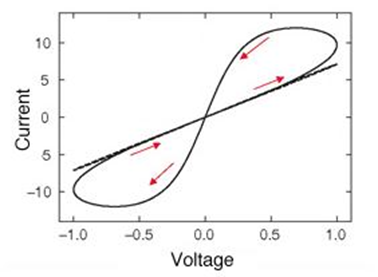
\includegraphics[width=0.5\textwidth]{Chapter1/Figs/1b.png}
\caption[Typical I-V characteristic of a memristor]{The typical I-V characteristic  of a memristor displays a pinched hysteresis loop resulting from the nonlinear relationship between current and voltage in memristance \cite{wen2012dynamics}.}
\label{fig:1b}
\end{figure}

\noindent The pinched hysteresis loop, which is characteristic and dependent on frequency, distinguishes these memristor devices from other components \cite{chua2019resistance}, as shown in Figure \ref{fig:1b}.  This loop is a common, natural phenomenon. As the voltage input frequency increases, the loop decreases in size. When the frequency is close to infinity, the memristor can be approximated as a resistor.

\subsection[Material Properties]{Material Properties}

Among the range of new non-volatile memory devices, the primary focus of this study is on memristor devices, including MRAM, PRAM, FeRAM, and RRAM \cite{wang2017memristors}. Resistive switching, a reversible phenomenon of two-terminal elements, characterises the devices. Through electrical signalling, they change resistance in a non-volatile manner, with the process driving the resistive switching defined by the device's materials \cite{mehonic2018silicon}. \\

\noindent Resistive random-access memory (RRAM) is a device that uses resistance switching, where reversibility is attained through repeated application of appropriate stimuli, according to \cite{liu2010controllable}. Repeated application of suitable stimuli ensures reversibility. An RRAM cell comprises an insulating thin film (usually a metal oxide), sandwiched between two electrodes, within which resistance switching occurs. \\

\noindent The term "memristance" is favoured to express the general characteristics of these RRAM devices. The central hypothesis of this model is that memristance is a function of the total charge that has been passed through the device or that the integral of the applied voltage is consistent with certain experimental data. This can be used to toggle between different resistance levels. Although this ideal memristor model is often used in RRAM cells, it may not satisfy practical requirements. \\

\begin{figure}[htbp!] 
\centering    
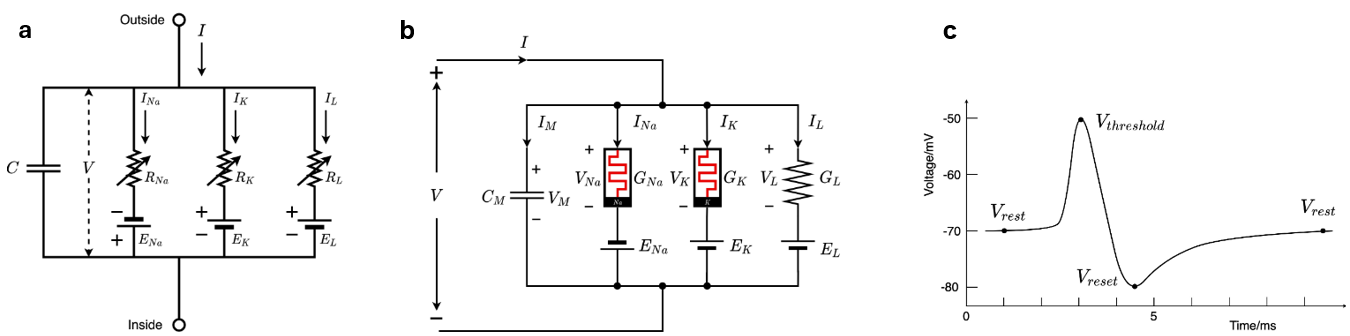
\includegraphics[width=0.8\textwidth]{Chapter1/Figs/1c.png}
\caption[The main RRAM types.]{The main RRAM types, from left to right: electrochemical metallization memory (ECM), vacancy change memory (VCM), and thermochemical memory (TCM). \cite{goux2016electrochemical}}
\label{fig:1c}
\end{figure} 

\noindent In normal operation, the state of the memristor can be objectively designated as having high resistance in the "OFF" state and low resistance in the "ON" state, with a substantial difference in resistance levels. The shift from the high resistance state (HRS) to the low resistance state (LRS) is referred to as "Set," while the reverse is called "Reset." An electroforming step is generally necessary to convert the device from pristine to switchable, whereby the former tends to exhibit higher resistance. \\

\noindent Although all RRAM devices operate on a metal-insulator-metal (MIM) architecture, their categorisation and analysis remain challenging. RRAM devices are loosely classified into two types based on their functional mechanisms: oxide-RAM (OxRAM) and conductive bridge RAM (CBRAM) \cite{liu2015categorization}. However, the internal physical behaviour of RRAM devices greatly varies, making it difficult to obtain a unified picture of them. RRAM cells may be classified according to their switching mechanisms which are electrochemical metallisation (ECM), valence change mechanism (VCM), or thermochemical mechanism (TCM) \cite{goux2016electrochemical}. The operation of the device is explained by one of the mechanisms depicted in Figure \ref{fig:1c}. \\

\paragraph{ECM:} The process of electrochemical metallisation (ECM) refers to the formation of a metallic conducting bridge in the electrolyte that connects two metallic electrodes. Generally, these electrodes comprise a conducting metal, like \textit{Ag} or \textit{Cu}, and the other is a chemically inert metal, like \textit{Pt} or \textit{TiN} \cite{waser2010nanoionics}.  The active layer typically consists of an ion conductor, solid electrolyte, or bulk isolator. The key factor driving these devices is the formation and breakage of \textit{Ag} or \textit{Cu} filaments in the active layer. During electroforming and "Set" processes, a positive bias is applied to the device, inducing anodic oxidation. Metallic cations originate from the active electrode and propagate through the insulating layer in the presence of an electric field. When the positive ions arrive at the inactive electrode, they undergo chemical reduction, leading to the production of filaments. If the electric field is strong enough to cause temperature-assisted atom diffusion and significant current-induced Joule heating, the filament is broken during the "Reset" phase.

\paragraph{VCM:} The valence change mechanism (VCM) describes the migration of oxygen vacancies, allowing carriers to tunnel between electrodes. VCM cells accommodate metallic electrodes that can be symmetrical or asymmetrical, with a metal oxide used as the insulating layer.  VCM cells accommodate metallic electrodes that can be symmetrical or asymmetrical, with a metal oxide used as the insulating layer. Examples of such metal oxides include \textit{$TiO_x, SrTiO_x, TaO_x,$} and \textit{$HfO_x$} \cite{lee2010evidence}. In this instance, the active electrode does not provide diffused metallic ions to create conducting filaments in the insulating layer. Instead, it is likely that oxygen vacancy migration is the primary switching mechanism for VCM devices. The device's symmetry is established following the initial forming step to form an n-type conducting channel located near the active electrode. Often, a tunnelling barrier exists between the electrode and the conductive channel. Fluctuations in the barrier height due to oxygen ion flow result in the production of different resistance states. During the "Set" procedure, oxygen ions are removed from this region. In contrast to the increased thermionic and tunnelling currents, the barrier height is decreased. These ions return to the vacant positions during the "Reset" process.

\paragraph{TCM:} Thermochemical memory (TCM) theory proposes that metal oxides with lower valencies are energetically preferred at higher temperatures. This energy difference induces the creation of a metal filament.  At higher temperatures, the oxide states with lower valencies have lower energy and are therefore favored. TCM devices have an insulating layer that can be made of NiO or $TiO_x$\cite{waser2009redox}. TCM devices typically operate with local stoichiometry that is dependent on the temperature gradient. This results in the movement of oxygen ions and vacancies along the temperature gradient, altering the switching position along the conductive pathway. The creation of conductive filaments can be altered irreversibly due to an increase in local temperature, leading to thermionic breakdown at high current levels. The formation of the filament is determined by the metal oxide. The injection of electrons at the cathode causes filament growth in n-type oxides, which subsequently progresses to the anode. Meanwhile, p-type oxides depend on anode contact hole injection, resulting in filament development in the opposite direction \cite{kim2011nanofilamentary}. \\

\noindent This study's devices and samples will employ silicon dioxide $SiO_x$ \cite{mehonic2012resistive} as their primary insulating layer material, in addition to electrode materials like $Ag$ or $Cu$. Since silicon-rich silica is commonly utilised as an insulating layer, it holds significant promise for CMOS-compatible processing.  To gain a better understanding of silicon oxide's characteristics, an electron injection model was developed \cite{gao2016mechanism}. \\

\noindent Within the amorphous structure of silicon oxide, $O-Si-O$ bonds are present, some of which possess wide-angle bonds that can function as profound electron traps, able to capture two electrons. The $Si-O$ bond is subsequently weakened once the broad bonds have captured both electrons, which lessens  the energy requirement to break the connection and produce the Frenkel defect. The creation of these imperfections leads to the formation of a group of voids, which can subsequently aid in the creation of the conductive filament.\\

\noindent In bulk silicon oxide, a conductive filament can form within the insulating layer during electroforming. The switching process is typically controlled by a single conductive filament, which is not affected by the electrode size.  The switching action leads to minor modifications to the filament. Since the resistance change usually takes place within a limited area, it is unrelated to the thickness of the insulating layer. \\

\noindent Contrastly, the filamentary switching, also called surface switching mechanism, is relatively unfamiliar. The electrode size significantly determines its conductivity.  This mechanism's operation primarily depends on Schottky tunnel barrier formation over the entire electrode contact and insulating layer, which produces a switching layer at the interface.

\subsection[Conduction Mechanisms]{Conduction Mechanisms}

How well a substance resists the flow of electrical charge is determined by its electrical conductivity, an inherent characteristic. An ideal insulator would have infinite resistance and zero conductivity.  However, a thin layer of silicon oxide that is just a few hundred nanometres thick has limited conductance and fall short of ideal electrical resistivity. \\

\noindent A range of external factors have the potential to affect the conductivity of the semiconductor material. These include the electric field applied, sensitivity to temperature and light frequencies.  The electric field strength, $E$, may be modelled by utilising the applied voltage, $V$, and distance across which the voltage is applied, d, giving the equation $E = \frac{V}{d}$. It should be noted, however, that this basic approximation may not be applicable to actual electronics. \\

\begin{table}[h]
\caption{Basic conduction mechanisms for insulators \cite{sze2021physics}.}
\resizebox{\textwidth}{!}{%
\begin{tabular}{ccc}
\hline
Process                      & Expression & Voltage \& Temperature \\ \hline
Conventional Tunnelling                   
& $J\propto E^{2} exp\left[ -\frac{4\sqrt{2m^{*}}(q\phi _{B})^{^{3/2}}}{3q\hslash E_{i}} \right] 
$  
& $J\propto V^2exp \left( -\frac{b}{V}\right)$  \\

Fowler-Nordheim Tunnelling 
&  $J = \frac{q^2E^2}{8\pi\hslash\phi _B} exp \left[  -\frac{4\sqrt{2m^{*}}(q\phi _{B})^{^{3/2}}}{3q\hslash E_{i}} \right ]$  
& $J \propto \frac{4\pi q m^* kT}{\hslash^3}$ \\

Thermionic Emission          
&  $J = A^{**}T^2exp \left[ -\frac{q(\phi _{B} - \sqrt{qE_i/4\pi \varepsilon _i} )}{kT} \right ]$          
&   $J \propto exp \left[ \frac{q}{Kt} \left( a\sqrt{V} - \phi _{B} \right ) \right]$ \\

Poole-Frenkel Emission       
&  $J \propto E_i exp \left[  -\frac{q(\phi _{B} - \sqrt{qE_i/\pi \varepsilon _i} )}{kT} \right ]$          
&  $J \propto V exp \left[ \frac{q}{kT} \left( 2a\sqrt{V} - \phi _{B} \right ) \right ]$  \\

Ohmic                        
&  $J \propto E_i exp \left( -\frac{\Delta E_{ac}}{kT} \right)$         
&   $J \propto exp \left( -\frac{c}{T} \right )$\\

Ionic Conductance            
&  $J \propto \frac{E_i}{T} exp \left(  -\frac{\Delta E_{ac}}{kT} \right )$         &   $J \propto \frac{V}{T}exp \left( -\frac{d'}{T} \right ) $   \\

Space-Charge-Limited-Current 
&  $J = \frac{9\varepsilon _i \mu V^2}{8d^3} $          
&   $J \propto V^2$ 
\\ \hline
\end{tabular}%
}
\label{table:1a}
\end{table}

\paragraph{Tunnelling:} Conventional tunnelling is the primary mode of conduction for insulating materials in high electric fields. Tunnelling, a quantum mechanical phenomenon, occurs due to the finite probability of the electron wave function passing through a potential barrier with limited height.  Conventional quantum tunnelling, on the other hand, refers to the instantaneous tunnelling of electrons across the entire width of the barrier. Table \ref{table:1a} illustrates the relationship between tunnelling current density and voltage as well as the dependence on electric field, while remaining independent of temperature. The variables used in the formula are $\phi_B$ for tunnelling barrier height, E for the insulator electric field, $m^*=0.42m$ for the carrier effective mass for silicon oxide, $\hslash$ for the reduced Planck constant, $q$ for electric charge, and $b$ for a constant factor of proportionality. Where technical terms are first used, their abbreviations are explained. 

\paragraph{Fowler-Nordheim Tunnelling:} Electron tunnelling through only a portion of the barrier height is recognised as Fowler-Nordheim tunnelling. The mechanism of Fowler-Nordheim tunnelling is determined by the trapezoidal shape of the potential barrier.  The application of a strong electric field results in more band-bending. As a result, the effective breadth through which carriers must tunnel is exponentially reduced. Fowler-Nordheim tunnelling is the primary conduction mechanism for metal oxide systems with thick oxide layers. After tunnelling through, the carriers are able to move freely between the conduction and valence bands. The straightforward requirement for tunnelling in this instance is that the electric field multiplied by the thickness of the layer exceeds the barrier height.

\paragraph{Thermionic Emission:} In general, thermionic emission is formed using a metal-to-insulator junction instead of a P-N semiconductor junction. This often leads to a negligible forward voltage drop and a swift switching action. It is important to ensure a clean surface for close contact between the metal and semiconductor during production. The fundamental relationships for thermally induced current are presented in Table \ref{table:1a}. Where $A^{**}$ represents the effective Richardson constant, $\epsilon$ denotes the permittivity of the insulator, and $a$ serves as a proportionality constant, the current is generated by the movement of charge carriers, which may be either electrons or ions, across a potential barrier that has been thermally excited. In order for such movement to occur, the carriers' thermal energy must exceed the material's work function. The current density's magnitude is directly proportional to the temperature.

\paragraph{Poole-Frenkel Emission:} Conduction may take place regardless of explicit quantum tunnelling through the insulator. In materials with a high density of structural defects, carriers are unable to travel as they would in tunnelling mechanisms. Owing to the presence of these structural flaws, additional energy states, or traps, emerge around the energy band margins. These traps limit the flow of electricity through a capture and release process. Electrons trapped in these states are dealt with by the Poole-Frenkel conduction mechanism. These trapped electrons can eventually accumulate sufficient energy to escape from isolated trap states due to thermal fluctuations in the material. If the electrons are not captured in another trap state, they will eventually reach the conduction band. Therefore, this mechanism is affected by both the applied electric field and the thermal energy. The electron's total energy arises from a combination of electric fields and temperature fluctuations. The electron's conduction process is primarily propelled by the electron drift current, $J = qn\mu E$, in which $q$ refers to the electric charge, $n$ represents the carrier density, $\mu$ denotes the carrier mobility, and E represents the electric field. The influence of trap depth $\phi_B$, insulator permittivity $\epsilon$, and temperature $T$ on this current can be demonstrated. To accommodate the fabrication approach and semiconductor materials utilized, an non-ideal factor $m$ that ranges between 1 and 2 may be incorporated in the equation.

\begin{figure}[htbp!] 
\centering    
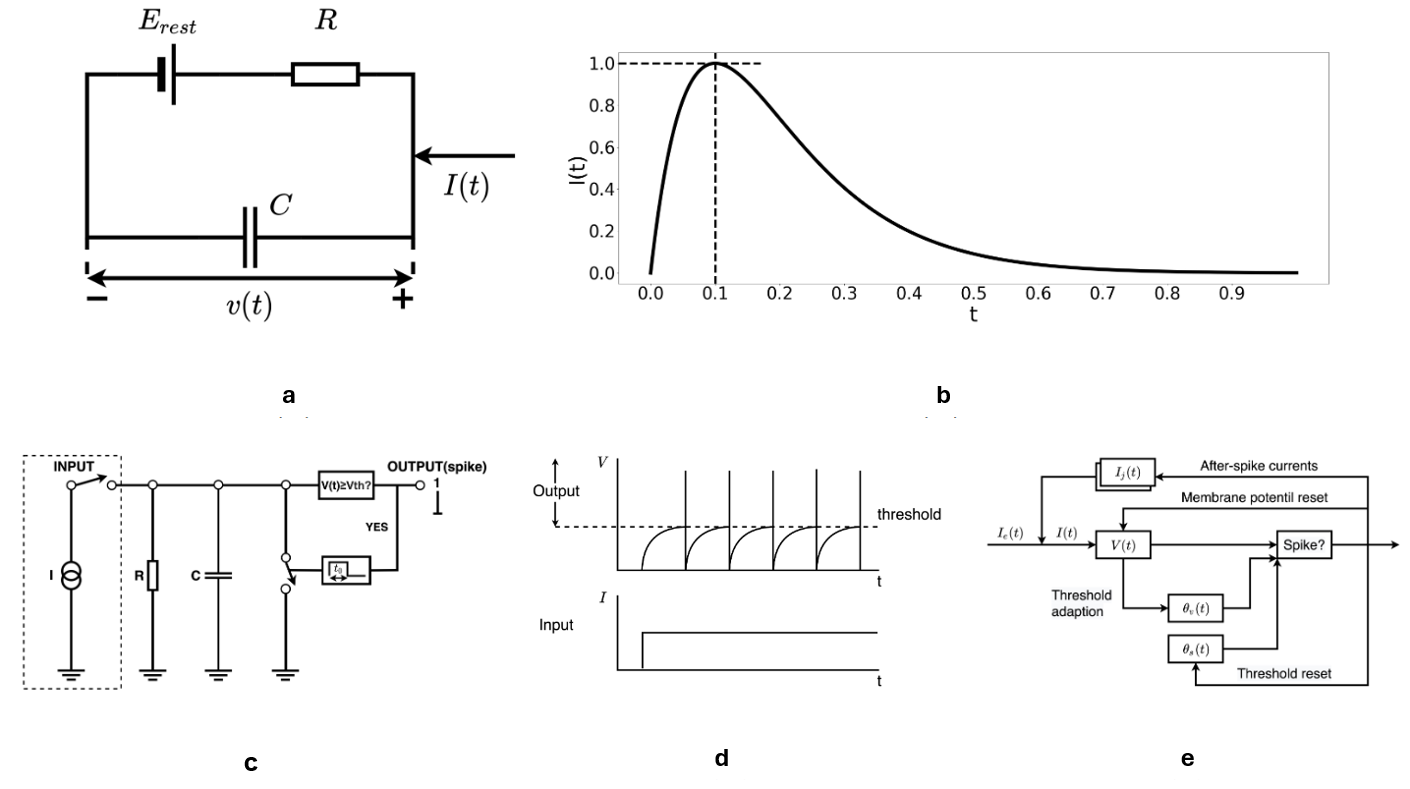
\includegraphics[width=0.6\textwidth]{Chapter1/Figs/1d.png}
\caption[Energy-band diagrams showing different conduction mechanisms.]{Energy-band diagrams showing different conduction mechanisms: (a) direct tunnelling, (b) Fowler-Nordheim tunnelling, (c) thermionic emission, (d) Poole-Frenkel emission, (e) trap-assisted tunnelling \cite{sze2021physics}}
\label{fig:1d}
\end{figure}

\noindent Other conduction mechanisms comprise Ohmic conduction, where the current density depends on the electric field, voltage, and temperature. In Ohmic conduction, $\Delta E_{ac}$ represents the activation energy, $k$ signifies the Boltzmann constant, $T$ denotes the temperature in Kelvin, and $c$ is a constant of proportionality. This type of conduction dominates at high temperatures and low fields since carriers change between conductive states due to thermal energy. Although ionic conduction has its own activation energy and proportionality constant, it shows comparable behaviour to ohmic conduction. This phenomenon can be described as ions moving through a substance via imperfections in the crystal lattice of a solid. \\

\noindent A flawless insulator hinders the mere ingress and egress of ions. Nonetheless, at the interfaces of metal-insulator, ionic carriers accumulate and alter the voltage distribution of the region under the influence of an electric field. Upon removing the applied electric field, a significant internal field remains, permitting the flow of an ionic current until an equilibrium state is reached. Finally, space-charge-limited current may arise from injected charge from the electrodes extending deeper into the insulator without compensating charges.\\

\noindent Charges are introduced to the dielectric material from one electrode and are subsequently removed by the other. The Mott-Gurney law is defined as $J=\frac{9\epsilon\mu V^2}{8L^3}$ and $J=\frac{2\epsilon vV}{L^2}$ for space charge limited current in solid and in the velocity-saturation regime, respectively. In this context, $\epsilon$ represents the dielectric permittivity, $\mu$ indicates the carrier mobility, $L$ denotes the material thickness, and $v = \mu E$ represents the electron drift velocity. With no inherent conductivity and a zero electric field at the cathode injecting charge, this mode of conduction necessitates the presence of a single type of charge carrier.\\

\noindent The tunneling processes described in the table above are based on a single-step process. However, defects within the insulating layer may allow for two or more tunneling phases, as shown in Figure \ref{fig:1d} (e). These structural flaws or traps may be generated during production or under stress from a high electric field. Consequently, the energy barrier may be fragmented in multiple ways if traps exist, thus increasing the likelihood of carriers tunneling through progressively thinner barriers.\\

\noindent Elastic or inelastic trap-assisted tunnelling may occur, either with or without energy dissipation in the carriers. In materials with a high density of structural imperfections, conduction is more probable in the presence of multiple oxide traps during the tunnelling process. A simpler equation linking tunnelling current density with trap barrier height has been validated at high electric fields for the case of trap-assisted tunnelling \cite{houng1999current}.

\subsection[Device Behaviours]{Device Behaviours}

After examining the physics that underlie the materials and mechanisms composing new RRAM devices, it is helpful to evaluate the general device behaviours concerning $I-V$ characteristics, volatility, polarity dependence, and power consumption to enhance application design. RRAM devices can respond in three ways \cite{li2017resistive}. \\

\begin{figure}[htbp!] 
\centering    
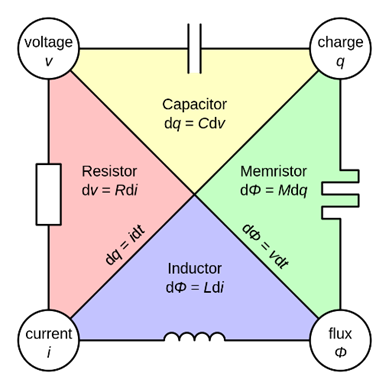
\includegraphics[width=1\textwidth]{Chapter1/Figs/1e.png}
\caption[Schematic I-V curves.]{Schematic I-V curves in: a) non-volatile bipolar memory switching mode, b) non-volatile unipolar memory switching mode; and c) volatile threshold switching mode. In the SET process, a compliance current is required to avoid hard breakdown \cite{li2017resistive}.}
\label{fig:1e}
\end{figure}

\noindent They are classified as unipolar if they are set and reset with the same polarity. When set and reset are accomplished with opposing polarities, the device is said to be bipolar. Moreover, threshold switching occurs when a device transitions to its low resistance state within a certain voltage range. Additionally, the term nonpolar designates devices that are polarity-independent, and thus, may perform both unipolar and bipolar operations. Figure \ref{fig:1e} summarises these three categories.

\paragraph{Bipolar Switching:} Bipolar switching entails configuring and resetting devices in polarities that oppose one another. The said behaviour has been noted in several oxide materials \cite{wei2008highly}. Current compliance is necessary for the setup of the switching mechanism, but the same applied current compliance can be used to reset it. The compliance system is notably simpler than that of the unipolar switching strategy. The switching voltage magnitude for bipolar devices falls within typical limits for digital chip integration. For instance, operational voltages can be below $\pm 1V$ in either polarity \cite{menke2009separation}. 

\paragraph{Unipolar Switching:} Unipolar switching, similar to bipolar switching, has been shown to occur in various oxide materials \cite{jeong2007coexistence}. In unipolar operation, electroforming and setting are driven by the electric field, whereas resetting is usually driven by current. To avoid competition between the two operating systems, a current compliance must be enforced during the setting process, as resetting is initiated by excessive currents. Once the device is configured, the current compliance can be augmented or eliminated entirely to enable adequate current flow and reset the device. The unipolar device's ability to operate with a single supply rail makes it compatible with digital integrated circuits. A significant drawback of these devices is the complex compliance system that is required, as the high reset current can generate heating and power usage issues, especially when scaling large memory arrays \cite{yun2007random}.

\paragraph{Threshold Switching:} Threshold switching happens when a device changes to a low resistance state once the applied voltage reaches a threshold and quickly returns to the previous state when the voltage falls below a lower threshold, displaying hysteresis \cite{adler1980threshold}. This occurrence was suggested as a consequence of thermal dissipation after assessing the diverse thicknesses of the bottom electrode \cite{chang2008effects}. This suggests that altering the electrode dimensions in the manufacturing process may result in different intended threshold switching behaviours. \\

\noindent Aside from the processes of switching, multiple aspects must be considered during the development of RRAM. Firstly, OxRAM samples typically exhibit a lower on/off conductance ratio within the range of 10s-100s and provide strong retention for up to $10^{12}$ cycles \cite{ielmini2010resistance}. On the other hand, CBRAM offers a relatively high on/off conductance ratio within the range of $10^3$-$10^6$, however, it has limited endurance to less than $10^4$ cycles \cite{ambrogio2014statistical1}. \\

\noindent The stochastic behaviour of oxygen or metal ions during ionic migration and the variability in filament form from device to device and cycle to cycle within a single device are unpredictable parameters that pose a significant challenge for the design of RRAM cells \cite{ambrogio2014statistical2}. Due to these variations, the density of RRAM prototypes ready for commercialisation is quite low at approximately 4 Mb. \\

\noindent Recent research has made significant progress in showcasing the capabilities of high-density devices with impressive features and low power consumption of approximately 0.1 pJ \cite{yang2013memristive}. Additionally, these devices have better reliability, with endurance exceeding $10^12$ cycles and retention of over 10 years at 150°C \cite{hu2014review}. They also exhibit higher density of 32 Gb through simpler fabrication steps and stronger thermal characteristics \cite{cha2013nanoscale}. This, coupled with the considerable resistance fluctuation not only among different devices but also within and between programming cycles on the same device \cite{moore2006lithography}, has engendered apprehension about the reproducibility of their electrical characteristics. \\

\noindent  These issues have prevented RRAM from commercialisation, despite its many appealing characteristics. Thankfully, the primary deep learning-based neural processing methods, such as regression, pattern recognition, and speech recognition, are random in nature and require less accurate computing than deterministic traditional computing. As a result of fewer impact from device variations during manufacture, compared to memory applications, on computation outcomes \cite{malik2013governing}, RRAM devices have generated additional possibilities to become suitable candidates for neural technologies. This can be attributed to the more tolerated necessity for variation in neural applications, alongside recent technical advancements.

\subsection[Compute Hardware Basics]{Compute Hardware Basics}

\noindent When discussing computer hardware, three key factors are essential: architecture, data representation, and method of computation. For instance, modern digital computers use the von Neumann architecture, represent data discretely, and perform computations using logic gates. The history of traditional computer architecture can be traced back to the 19th century when the concept of mathematical computing devices was first introduced \cite{bromley1982charles}. The primary reason for this separation was complexity. Memory and computation units are challenging to design individually, so it made sense to separate them while still allowing communication between them. \\

\noindent John von Neumann popularised this approach, which became the norm with the emergence of the first electronic computers in the 1940s \cite{von1993first}. However, this architecture can lead to the so-called von Neumann bottleneck. In many applications, data must be retrieved from memory and moved to computing units for the execution of mathematical operations, such as multiplication and addition, before being stored back in memory. If the application is data-intensive, a significant amount of time and energy is spent on transferring data between memory and compute units, rather than on the actual computations. \\

\noindent Data representation is a crucial aspect of modern computing, and it has been largely defined by the concept of the Turing machine. Alan Turing's work laid the foundation for programming, which is the idea that a machine can implement arbitrary algorithms \cite{turing1936computable}. However, this relies on machines operating on precisely identifiable states, which in practice means discrete data representation. The approach of digital computation also determined how calculations are performed in hardware. \\

\begin{figure}[htbp!] 
\centering    
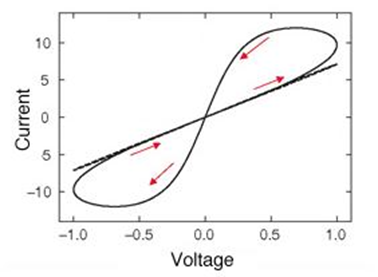
\includegraphics[width=0.5\textwidth]{Chapter1/Figs/1f.png}
\caption[Full Adder Circuit.]{In the full adder circuit, $A$ is the operand to be added, and $B$ is the operand being carried forward. $C_\mathrm{in}$ is the carry forward bit of the previous addition, and $S$ is the total. The carry bit of the next addition is $C_\mathrm{out}$.}
\label{fig:1f}
\end{figure}

\noindent Logic gates are the fundamental components of digital computers. The theory of logic circuits was developed in parallel with the conceptualisation of the Turing machine. Building on the work of George Boole, Claude Shannon and others \cite{shannon1938symbolic}, switching circuits were designed to solve arbitrary problems in Boolean algebra. The basic elements of these circuits, known as logic gates, were initially implemented using mechanical relays, vacuum tubes, and later transistors. However, even simple operations can require a large number of devices. For instance, a full adder circuit in figure \ref{fig:1f}, adds two binary numbers and a carry bit, requiring 26 transistors \cite{raghunandan2019design}. Adding more bits necessitates more transistors, increasing energy consumption and circuit area. \\

\noindent There are several levels to compute optimisations in a digital computer. At the most basic level, the number of transistors in a computer can be reduced to allow for the implementation of more complex circuits in the same space. Different decisions can be made regarding the operations that those transistors are required to carry out; this is commonly known as instruction set architecture (ITS). The broadest instruction sets result in the most general purpose processors, such as the central processing unit (CPUs). Conversely, the narrower instruction set which results in implementations such as the graphics processing unit (GPUs), can lead to better performance in specific applications. \\

\noindent At a structural level, the conventional von Neumann architecture remains difficult to phase out, but there have been efforts to unify memory and computation even within the digital paradigm. For example, microcontrollers have a single chip that consolidates both computation and memory. Similarly, many cutting-edge AI chip designs aim to pack the maximum number of computational elements and memory units onto a single chip. \\

\section[In-memory Computing Paradigms]{In-memory Computing Paradigms}

As improvements at the device level in digital computers become increasingly difficult, alternative computing paradigms offer a more promising direction. Specifically, targeting the memory bottleneck mentioned earlier could bring significant benefits. The Von Neumann architecture results in slow and energy-inefficient data movement, which is even more pronounced today, as data-intensive applications like machine learning gain popularity. Bringing memory and compute units closer together, ideally achieving in-memory computing (IMC), could alleviate the problem. \\

\noindent Proposed solutions for addressing the von Neumann bottleneck vary. These include digital and analogue approaches, which can be differentiated based on the integration level between memory and computing units. The conventional von Neumann architecture, which completely separates memory and compute units, represents one end of the spectrum. In the pursuit of IMC, there are techniques that involve placing memory and compute units on the same chip. \\

\noindent One such technique is near-memory computing, which integrates embedded non-volatile memories (NVMs) into microcontrollers. In this approach, NVM is used to store model parameters, while volatile memory, such as SRAM, is sandwiched between NVM and compute units to hold intermediate input/output data. \\

\noindent In a true IMC approach, memory serves a dual purpose: storing data and performing computations. To achieve general-purpose computing in memory is incredibly challenging; therefore, a more realistic approach is to focus on specific applications. For instance, in the field of machine learning, the objective may be to expedite linear algebra computations. \\

\noindent One commonly used approach for IMC is the utilization of resistive crossbar arrays. In this approach, neural network weights are represented using analogue properties, such as device conductance. The underlying physics, together with the circuit structure, can then perform the necessary computations. This is achieved without the need to move the weights from memory to compute units, as the weights (in the form of conductances) are directly operated on by applying physical stimuli, such as voltage, to them.

\subsection[Recent Development]{Recent Development}

Computers based on the von Neumann architecture and the complementary metal-oxide semiconductor (CMOS) technology are now ubiquitous due to their scalability, which has resulted in multi-decade improvements in speed and space efficiency. However, the slowing down of Moore's law and the increasing costs in data-intensive applications such as machine learning are becoming prohibitive. For instance, it has been reported that programs such as ChatGPT have high training and inference costs \cite{mok2023chatgpt}. This could be a factor in their reduced performance \cite{chen2023chatgpt}, as minimising expenses may be prioritised. \\

\noindent Modern computer designs reflect the well-known issue of memory bottlenecks. Large volumes of data are stored in off-chip memory, such as dynamic random-access memory (DRAM), while frequently accessed data are stored in on-chip memory, such as static random-access memory (SRAM), which is located closer to the compute units. \\

\noindent On-chip memory can be more than 100 times more energy efficient than off-chip memory, but it is also more costly and requires more space \cite{han2016eie}. That is difficult in the case of machine learning since the models being trained are so huge. Without compression, even models from ten years ago cannot fit into ordinary SRAM units, necessitating the use of more energy-intensive DRAM \cite{han2015deep}.\\

\noindent Additional enhancements to the compute units can be realised following memory optimisation. CPUs are the most general-purpose calculation units, supporting a wide range of instructions and operating in a sequential order. They can be made more parallel by adding more cores, but whether this is effective depends on the application. \\

\noindent GPUs are more specialised, with a concentration on graphics processing, although they can perform a wide range of matrix operations. They are also more parallel than CPUs, but they can only execute a limited number of instructions and control flow. Tensor processing units (TPUs) are compute units created expressly with machine learning in mind; optimisations are made for matrix multiplication, data retrieval, and even instruction fetching \cite{jouppi2017datacenter}. \\

\noindent Finally, device developments have tended to focus on lowering transistor sizes, resulting in higher density and speed. This general tendency (known as Moore's law) has resulted in transistors that are just a few nanometers in size. Commercial manufacturing of 5 nm transistors began in 2020, with deployments in Apple, Qualcomm, Huawei, Marvell, and Nvidia consumer products \cite{wang2022tsmc}. \\

\noindent 3nm transistor manufacture began in 2022, although widespread commercialization has yet to occur. Continuous transistor size decreases are extremely difficult and expensive to produce, with diminishing advantages. Moore's law (in its classic version) is not likely to continue indefinitely due to physical limitations—even now, the tiniest transistors may be just a few tens of atoms thick in certain directions.


\subsection[Original Implementation]{Original Implementation}

Linear algebra and vector-matrix products rely heavily on multiplication and addition. These procedures can be carried out by using fundamental circuit laws. Consider a resistive element with conductance $G$ (the reciprocal of resistance). If a voltage $V$ is supplied to it, the current $I$ flowing through it will be equal to $V \times G$. This indicates that conductance $G$ functions as a multiplicative factor, as per Ohm's law. For a circuit with several branches, each carrying a current $I_i$. At the intersection of these branches, the total current flowing through it will be $I = \sum_{i}^{} I_i$. This indicates that currents are combined together, as per Kirchhoff's current law. \\

\noindent Once multiplication and addition are possible, higher-level operations may be performed using specialist circuits. For vector-matrix products, a resistive crossbar array can be used, which is a two-dimensional grid of conductive wires with resistive components at each intersection. A crossbar array's output currents are essentially the product of a voltage vector and a conductance matrix. Consider a vector-matrix product, $\mathbf{y} = \mathbf{x}^\intercal \mathbf{W}$. Where $\mathbf{x}$ can be translated to voltages $\mathbf{V} = k_V\mathbf{x}$, $\mathbf{W}$ to conductances $\mathbf{G} = k_G \mathbf{W}$, and generate outputs $\mathbf{y}$ from currents $\mathbf{I} = \mathbf{y} k_V k_G $, where $k_V$ and $k_G$ are positive constants. \\

\begin{figure}[htbp!] 
\centering    
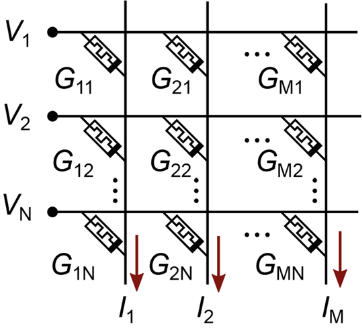
\includegraphics[width=0.5\textwidth]{Chapter1/Figs/1k.png}
\caption[The memristor-based crossbar architecture.]{The memristor-based crossbar architecture with a single memristor array and a constant-term circuit \cite{truong2014new}. The resistive components are located at the connections of the word and bit lines. When voltages $\mathbf{V}$ are applied to the word line, the resistive element at the junction of the $i^{th}$ word line and the $j^{th}$ bit line generates $V_i \times G_{i,j}$ units of current, assuming zero wire resistance, as per Ohm's law. The currents created by each individual element are then aggregated along the bit lines using Kirchhoff's current law.}
\label{fig:1k}
\end{figure}

\noindent Crossbars can compute products of voltage vectors and conductance matrices due to their structural design. This is because the structure controls which voltage-conductance pairs are multiplied and which consequent currents are combined together. These circuits have two sets of wires: word lines and bit lines. Voltages $\mathbf{V}$ are applied to the word lines, and currents $\mathbf{I}$ are measured along the bit lines. A resistive element located at the junction of the $i^{th}$ word line and the $j^{th}$ bit line has a conductance of $G_{i,j}$.\\

\noindent When $V_i$ is applied to the $i^{th}$ word line, the device generates a current of $V_i \times G_{i,j}$ (assuming no wire resistance). The currents generated in the jth bit line are added together to provide a current of $I_j$. This current is calculated by taking the dot product of voltage $\mathbf{V}$ and the $j^{th}$ column of the conductance matrix $\mathbf{G}$. Given that the $j^{th}$ element of a vector-matrix product is just the dot product of the vector and the $j^{th}$ column of the matrix, the vector containing all output currents may be concisely expressed as $\mathbf{I}^\intercal = \mathbf{V}^\intercal \mathbf{G}$. \\

\noindent The individual application determines which resistive devices are used in the crossbar array. Weights $\mathbf{W}$ are repeatedly updated during neural network training, necessitating the ability to alter the conductances in the crossbar array numerous times. In contrast, during inference, the weights are fixed, allowing the conductances to be set after initial programming. Regardless of the conditions, the conductances will be unique to the network, requiring the ability to change them at least once. \\

\noindent Memristive devices, or memrisitors, are differentiated by their ability to change their conductance in response to electrical inputs. As a result, they make an excellent choice for crossbar-based linear algebra accelerators. The choice of memristor depends on whether the crossbar array is used for training or inference. The former is far more difficult and would demand memristors that can be repeatedly programmed in a linear fashion. Given these complications, much research on memristive crossbars has been on inference. \\

\noindent Even in the absence of nonidealities, any memristor will have a restricted range of conductance values that it can be configured to. This is a hurdle when attempting to represent real numbers with solely positive conductances $G$. To demonstrate, if the range of attainable conductances is $G \in [G_{off}, G_{on}]$, the crossbar array can only represent matrix values up to $w \in \left [ \frac{G_{off}}{k_G}, \frac{G_{on}}{k_G} \right ]$. Since $G_{off}$ is a positive number, hence only positive $w$ may be expressed. \\

\noindent One potential option is to employ differential pairs, in which the matrix element $w$ is represented as the difference between two conductances, $G+$ and $G-$ \cite{joksas2022nonideality}. The two conductances can be chosen symmetrically around the 'average' value $G \pm = G_{avg} \pm \frac{k_G w}{2}$, where $G_{avg} = \frac{G_{off} + G_{on}}{2}$. The two sets of conductances can be represented by independent conductance matrices $\mathbf{G}+$ and $\mathbf{G}-$, which are assigned to different bit lines of the crossbar array \cite{kim20214k}. \\

\noindent The bit lines will then generate independent sets of currents, which may be represented as vectors $\mathbf{I}+$ and $\mathbf{I}-$. Vector-matrix products are linear, thus the result may be calculated by subtracting $\mathbf{I}-$ from $\mathbf{I}+$. In reality, the 'positive' and 'negative' bit lines are frequently arranged near to one another, which helps to mitigate the detrimental effects of line resistance, a significant non-ideality \cite{joksas2020committee}. 


\subsection[Memory Cells]{Memory Cells}

It is critical to understand the viability of various technologies for IMC systems. When volatile memory is used for computing, the computational parameters are often acquired from nonvolatile off-chip memory, which adds cost to overall system performance. The goal is to install IMC directly on NVMs, which would further minimise data travel, increasing energy efficiency and lowering latency. \\

\noindent One prospective path to explore is the use of mature Flash technology as a computational NVM. However, developing memory technologies have several advantages, including interoperability with increasingly powerful processor nodes. This is mostly owing to the lower operating voltages compared to Flash technology. Furthermore, several of these emerging technologies provide multi-bit or even fully analogue programmability \cite{mannocci2023memory}. This may be used to conduct multiply-accumulate operations in the analogue domain, resulting in additional performance advantages. \\

\noindent In a broader context, irrespective of the IMC concept, it is crucial to recognise that contemporary computing systems utilise a range of memory technologies, which are typically organised in a hierarchical structure. These memory technologies, which operate within the digital paradigm, are based on mature complementary metal–oxide–semiconductor (CMOS) fabrication and technology. \\



\begin{table}[h]
\caption{Benchmark of emerging memory technologies for various applications. \cite{molas2021advances}.}

\resizebox{\textwidth}{!}{%
\begin{tabular}{cccccccccc}
\hline
               & \begin{tabular}[c]{@{}c@{}}STT MRAM\\ SCM/DRAM\end{tabular}   & \begin{tabular}[c]{@{}c@{}}Embedded\\ MRAM\end{tabular}   & \begin{tabular}[c]{@{}c@{}}SOT\\ Cache\end{tabular} & \begin{tabular}[c]{@{}c@{}}Standalone\\ PCM\end{tabular} & \begin{tabular}[c]{@{}c@{}}Embedded\\ PCM\end{tabular}                 & \begin{tabular}[c]{@{}c@{}}Standalone\\ RRAM\end{tabular}    & \begin{tabular}[c]{@{}c@{}}Embedded\\ RRAM\end{tabular}              & FeRAM                                                                                      & FeFET                                                            \\ \hline
Capacity       & \textgreater{}1Gb                                             & 10-100Mb                                                  & \textgreater{}1Mb                                   & Gb                                                       & 10-100Mb                                                               & $\sim$1Gb                                                    & 1-10Mb                                                               & Poor                                                                                       & Small                                                            \\
Scalability    & Medium                                                        & Medium                                                    & Poor                                                & Good                                                     & Good                                                                   & Medium                                                       & Good                                                                 & Medium                                                                                     & Poor                                                             \\
MLC            & No                                                            & No                                                        & No                                                  & Possible                                                 & Possible                                                               & Theoretical                                                  & Theoretical                                                          & Theoretical                                                                                & Theoretical                                                      \\
3D Integration & No                                                            & No                                                        & No                                                  & Yes                                                      & Yes                                                                    & Yes                                                          & Yes                                                                  & No                                                                                         & No                                                               \\
Architecture   & Crossbar                                                      & Crossbar                                                  & 3 Terminals                                         & Crossbar                                                 & 1T1R                                                                   & Crossbar                                                     & 1T1R                                                                 & 1T1R                                                                                       & 3 Terminals                                                      \\
Retention      & \textgreater{}1yr 100°C                                       & 10yrs 150°C                                               & 85-100°C                                            & 85-100°C                                                 & Automotive                                                             & 10yrs 85°C                                                   & 10yrs \textgreater{}85°C                                             & 85-100°C                                                                                   & \begin{tabular}[c]{@{}c@{}}SMT\\ Compliant\end{tabular}          \\
Latency        & 10ns                                                          & 10ns                                                      & \textless{}ns                                       & 100ns                                                    & 100ns                                                                  & 100ns                                                        & 100ns                                                                & \textless{}20ns                                                                            & 5ns                                                              \\
Power          & pJ/bit                                                        & pJ/bit                                                    & fJ/bit                                              & 10pJ/bit                                                 & \begin{tabular}[c]{@{}c@{}}10pJ/bit\\ \textgreater{}200uA\end{tabular} & 1-10pJ/bit                                                   & \begin{tabular}[c]{@{}c@{}}1-10pJ/bit\\ $\sim$100uA\end{tabular}     & 10fJ/bit                                                                                   & 10fJ/bit                                                         \\
Endurance      & $10^{10}$                                        & $>10^6$                       & $>10^{10}$               & $10^7$                                    & $10^6$                                                 & $10^7$                                       & $10^6$                                               & \begin{tabular}[c]{@{}c@{}}$>10^{11}$\\ destructive\end{tabular} & $10^4-10^5$                    \\
Issues         & N/A                                                           & N/A                                                       & N/A                                                 & Drift                                                    & Drift                                                                  & \begin{tabular}[c]{@{}c@{}}Variability,\\ Noise\end{tabular} & \begin{tabular}[c]{@{}c@{}}Variability,\\ Noise\end{tabular}         & \begin{tabular}[c]{@{}c@{}}Small Size\\ Variability\end{tabular}                           & \begin{tabular}[c]{@{}c@{}}Small Size\\ Variability\end{tabular} \\
Space          & DRAM                                                          & NVM                                                       & Cache                                               & SCM                                                      & MPU,MCU                                                                & SCM                                                          & MPU,MCU                                                              & DRAM                                                                                       & Flash                                                            \\
Maturity       & \begin{tabular}[c]{@{}c@{}}Everspin,\\ Avalanche\end{tabular} & \begin{tabular}[c]{@{}c@{}}Avalanche,\\ TSMC\end{tabular} & No Products                                         & \begin{tabular}[c]{@{}c@{}}Intel,\\ Micro\end{tabular}   & \begin{tabular}[c]{@{}c@{}}ST\\ Microelectronic\end{tabular}           & No Products                                                  & \begin{tabular}[c]{@{}c@{}}Panasonics,\\ Dialog,\\ TSMC\end{tabular} & \begin{tabular}[c]{@{}c@{}}Texas Instruments,\\ Fujitsu,\\ Cypress\end{tabular}            & Good                                                             \\ \hline
\end{tabular}%
}
\end{table}

\noindent In the majority of cases, electrical charge is employed as a surrogate for data, and these are designated as charged-based memories. Fast volatile memory, such as static random-access memory (SRAM), represents the pinnacle of this hierarchical structure. It has the shortest access time, but is also characterised by low area density and typically the highest cost. \\

\noindent The middle of the hierarchy is typically occupied by off-chip DRAM, which serves as the main memory. It exhibits superior area density but experiences a slight extension in access time. At the lowest point of the hierarchy, there are   NVM technologies such as flash memory (in solid-state drives, or SSDs) and hard disk drives (HDDs), which possess the highest area density but are significantly slower. In this memory hierarchy of computing systems, emerging NVM technologies are seen as a means of bridging the performance gap, particularly in terms of speed, between the extremes of the hierarchy. \\

\noindent The most promising emerging memory technologies include resistive random-access memory (RRAM), phase-change memory (PCM), ferroelectric random-access memory (FeRAM), magnetic random-access memory (MRAM), spin-transfer torque magnetic random-access memory (STT-MRAM), and ferroelectric field-effect transistor (FeFET). It should be noted, however, that this is not an exhaustive list. There are other promising technologies under exploration and rapid development, such as electrochemical random-access memory (ECRAM) \cite{mannocci2023memory}, which could offer further computational performance benefits. \\

\noindent In order to provide a comprehensive overview, we will briefly address the physical mechanisms that underpin the operation of these memory technologies. Regardless of the specific technology under consideration, in addition to the typical requirements of NVM, the crucial enabling factor for executing linear algebra operations using, for instance, crossbar arrays is the ability to effectively configure a single memory cell into multiple stable, non-volatile memory states. \\

\noindent A resistive random-access memory (RRAM) cell is typically structured on a metal – insulator – metal basis, with the central insulating layer serving as a resistance-switching layer. This layer is typically composed of metal oxides, although other materials, including chalcogenides, organic substances, nitrides, and two-dimensional (2D) materials, are also being investigated. \\

\noindent Furthermore, a distinction can be made between filamentary and interface-based switching. This differentiation depends on whether the write operation results in the formation of conductive filaments within the insulating environment, or if the resistance switching is based on modulating barrier heights (for example, Schottky barriers) between the switching layer and the electrodes (metals). \\

\noindent A PCM cell shares certain similarities with an RRAM cell; however, the switching layer in PCM is composed of phase-change materials. These materials possess the capacity to reversibly transition from a crystalline to an amorphous phase. A representative example of a phase-change material is chalcogenide (such as $Ge_2 Sb_2 Te_5$), wherein the phase transition is driven by Joule heating generated by voltage pulses applied across the cell. \\

\noindent In addition to the two separate states, RRAM and PCM may also store intermediate states. This can be accomplished by either changing the shape of the conductive filaments (as in RRAMs) or adjusting the fraction of material that transitions between the two separate phases. This functionality is particularly useful in the context of analogue or multi-bit computing. However, other obstacles remain, including the accuracy and feasibility of programming several intermediate states, as well as their preservation. \\

\noindent Ferroelectric random-access memory (FeRAM) and ferroelectric field-effect transistors (FeFET) are both based on the use of ferroelectric effects. Typical examples of ferroelectric materials for FeRAM are perovskites. However, recent research has demonstrated significant interest in employing ferroelectricity from HfOx-based materials \cite{mulaosmanovic2021ferroelectric} (either doped or undoped) due to their superior compatibility with complementary metal-oxide semiconductor (CMOS) technology. \\

\noindent In the case of FeRAM, the state is read by measuring the displacement current during switching in the ferroelectric material, which is a destructive process and not ideal for computing applications. Alternative strategies include ferroelectric tunnel junctions (FTJs) and three-terminal FeFETs. In these cases, the states are read either as resistance or a threshold voltage. As a result, the read process is non-destructive and better suited for computing systems. \\

\noindent MRAM uses the magnetoresistive phenomenon to store data. The cell structure is similar to that of RRAM and PCM, but MRAM has two ferromagnetic layers, each capable of holding a magnetic field and separated by a thin tunnel layer. One of the ferromagnetic layers has a constant magnetic orientation, whilst the other layer may change its magnetic orientation to be parallel (aligned) or anti-parallel (anti-aligned) relative to the fixed layer. The first represents a logical '0', and the second represents a logical '1'. The state is determined by measuring resistance, as the two configurations produce different resistances due to magnetoresistance effects. \\

\noindent Currently, the two most common MRAM implementations are STT-MRAM and spin-orbit torque magnetic random-access memory (SOT-MRAM). The cell architecture of both implementations are identical, with the key variation being the approaches used to program the cell state. In the case of STT-MRAM, the magnetic orientation of the 'free layer' may be changed using spin torque, which transmits current pulses across the tunnel junction. In contrast, in SOT-MRAM, the transition to a new state is triggered by applying a current pulse down the heavy metal line (such as platinum or tantalum) on which the tunnel junction is formed. The current pulse causes the buildup of spin-polarized electrons, which switches the magnetisation of the free layer. \\

\noindent As previously noted, the notion of ECRAM has received significant attention in recent years. The ECRAM structure is similar to a transistor, with an extra vertical stack of a reservoir layer and a solid-state electrolyte. The insertion of ionised defects into the reservoir layer has the potential to change the channel conductivity. These flaws are often oxygen vacancies or lithium ions, although they may also comprise other species, such as protons. ECRAM has the potential to outperform other NVMs in terms of cycling endurance and linear conductance modulation control. This linear conductance modulation is frequently used in machine learning applications, particularly during training. \\

\noindent Memtransistors are a more contemporary idea that combines a three-terminal transistor shape with memristor-like functionality. This makes it easier to modify the channel's conductance by applying significant source-drain voltages. These devices often utilise two-dimensional semiconductor materials, such as MoS2, for their channel. Compared to the other NVM technologies discussed, memtransistors are still in the early phases of development. 

\subsection[Neural Processors]{Neural Processors}

Advances in ANN implementation and system speed, which prompted modifications in computer architectures, have resulted in improvements not just in software but also in hardware \cite{indiveri2015memory}. To run neural networks, many forms of hardware were used, including standard computers, neural accelerators, and neuromorphic computing \cite{majumdar2012massively}. \\


\noindent In reality, neuromorphic computers are becoming the most effective means of running neural networks, which necessitate whole other kinds of compute equipment, hence the names "neuromorphic chips" or "neural processing units" (NPUs). The number and structure of computational cores distinguishes central processing units (CPUs), graphics processing units (GPUs), and neural processing units (NPUs) \cite{taha2013exploring}. \\

\noindent In comparison to traditional CPUs, which are now sold with up to tens of cores, NPUs and GPUs have been claimed to contain over several thousand cores \cite{gupta2011performance}. Despite major variations in operations and organizations, there are numerous commonalities between NPUs and GPUs since they both use many cores for parallelizing neural network workloads, which may be found in image processing jobs. GPU cores, like CPU cores, serve primarily as processing units and lack memory capabilities. \\

\noindent This already takes into consideration the existence of SRAMs, which mostly served as caches. This suggests that GPUs require external memory to work, indicating that the GPU processor and memory are fundamentally independent functions. The primary difference between the core architectures of both CPUs and GPUs versus those of NPUs is that the latter are built with cores that have their own memory units, or synapses, that can perform neural network operations \cite{qiao2015reconfigurable}. \\

\noindent Thus, NPUs are capable of working with memory and processing concurrently under the same calculation, which is inspired by and extremely comparable to that of the human brain. Many contemporary NPUs use SRAM and DRAM as synapses, which are volatile components. This suggests that extra storage devices, such as flash drives or storage devices with non-volatile characteristics, are still required to maintain their synaptic weights, even though their processing and memory operations are connected \cite{chen201865nm}. \\

\begin{figure}[htbp!] 
\centering    
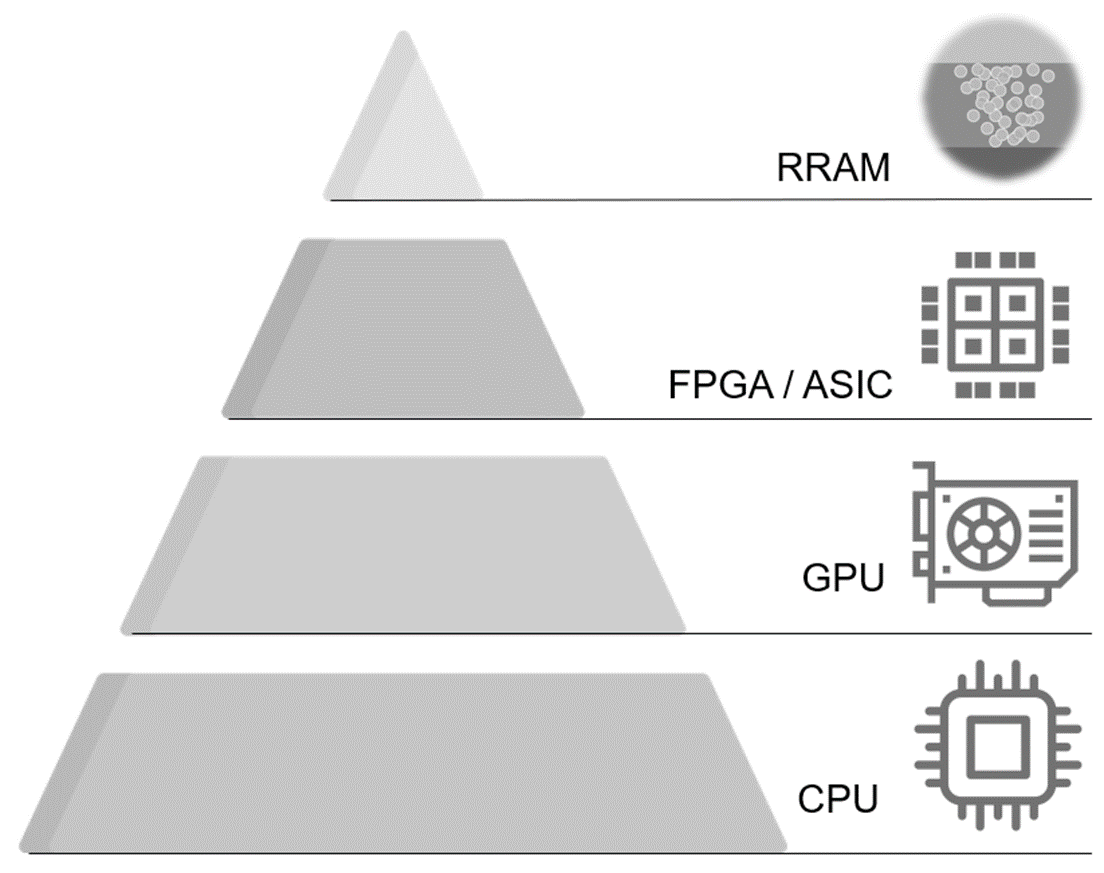
\includegraphics[width=0.5\textwidth]{Chapter1/Figs/1l.png}
\caption[Typical hardware technologies for DNN acceleration.]{Typical hardware technologies for DNN acceleration. Specialized hardware for high-performance DNN training and inference is included in the pyramid's top layer. RRAM is the name of the apex, although the term is meant to include all programmed non-volatile memristive devices.}
\label{fig:1l}
\end{figure}


\noindent The implementation of memristive devices as non-volatile synapses can reduce the need for external storage in order to have concurrent processing and memory during computation \cite{kim2015exploiting}. In order to dramatically reduce energy consumption and information congestion during data transfer across memory devices and processing components, NPU designs have continued to investigate the interconnected capabilities between processing and memory \cite{lee2013rmss}.\\

\noindent The ideal neural chip should have massively parallel processing capacity for bit-wise, fixed-point, and floating-point calculations of many different data sizes; low memory latency; memory bandwidth hundreds of times greater than what is obtainable in today's desktop devices; a remarkable memory size capable of handling big data; and a novel architecture that allows flexible and rich interconnection between memory and computing. \\

\noindent Each of the aforementioned requirements should be fulfilled while also taking into account reduced power consumption and increased energy efficiency. This makes it possible to create neural network units in circuit designs within NPU cores. According to the following general operating theory, the input neuron in the first layer can take a data input from the pre-synaptic neurons, perform matrix vector multiplication (MVM) with synaptic weights, and then produce another value for the hidden neurons. \\


\noindent These hidden neurons will act as input data for the subsequent neuron layer and then output neurons. Multiplication, addition, and activation have traditionally been the roles of the input and output neuron layers. While the weight storage capability of synapses may be implemented in memristors to retain the updated weights, these processes can be accomplished using CMOS electronic or analogue circuitry. In this view, weight storage becomes the main purpose of conventional synaptic structures \cite{schemmel2008wafer}. \\

\noindent Up to this point, only the use of memristive devices for weight storage has been considered, which remains the most prevalent option for practical NPUs. The most recent study is presently focusing on ways of more effectively and innovatively utilising memristors by leveraging the particular nonlinear $I-V$ characteristics of memristive devices. \\

\noindent It has been investigated whether the traditional method of matrix-vector multiplication, in which matrix components store analogue attributes or multi-level device values, can improve the effectiveness of ANNs by expanding synaptic devices' capabilities beyond their use in basic weight storage in ANN. \cite{wu2012alox}. The memristive crossbar array can effortlessly perform matrix-vector multiplication and naturally convert the weighted mixture of input signals to output signals, reducing the computational cost to $O(1)$ from $O(n^2)$. \\

\noindent To create a memory-sensitive crossbar that can conduct analogue multiply-accumulate (MAC) actions in a single time interval, a variety of device fabrication techniques may be used \cite{rahimi2020complementary}. In a non-von Neumann architecture, doing multiplication at the memory cross-point can result in an immediate decrease in temporal complexity. Under this widely used strategy \cite{xia2019memristive}, MVM may be parallelized with the vector denoted with $N$ as the size of the input voltage signals $[V_1,V_2,...V_N]$. \\

\noindent The crossbar rows are subjected to these voltages, and the size of the matrix is $(N x M)$. Its weights are kept in the memristive element at each cross point and are expressed as conductances. By using the fundamental Ohm's equation $I=V.G$, the current accumulated at each horizontal column represents one component of the resulting multiplication vector of length $N$.\\

\noindent Extra logic electronics, such as multipliers and adders, are not necessary for this matrix-vector multiplication approach because of the special characteristics of memristive devices, which enable them to automatically conduct multiplication and addition concurrently. The memristor may efficiently perform the functions of weight storage, multiplier, and adder throughout the process \cite{perez2016impact}. \\

\noindent The memristive device has to have appropriate conductance to voltage proportionality to support such operation \cite{merced2016repeatable}. This methodology may be extended to do matrix-vector multiplication and train neural networks \cite{sheridan2017sparse}. This variable resistance technology, which enables neural networks to be controlled via MVM in neural processors, is poised to make memristive devices particularly ideal for enabling it. \cite{xia2017mnsim}. \\

\noindent Memristors for MVM are much easier to construct than weight-storing methods \cite{hasan2016high}. It has frequently been claimed that using NPUs for computation is much more efficient than using conventional processing elements. This more intense MVM technique produces incredibly effective processing. \cite{courbariaux2016binarized}. \\

\noindent The MVM method is, in essence, the most effective technique to employ memristors as neural network synapses. However, there are still issues with real-world applications that need analogue properties or enough multi-levels of memristive devices to support machine learning for efficiency.

\subsection[Hardware Accelerators]{Hardware Accelerators}

Meristive devices have been used as weight components in many studies' neural network designs \cite{sidler2016large} in order to meet the two aforementioned main requirements for deep neural network acceleration: huge parallelism and decreased memory access \cite{azghadi2016hybrid}. This adaptive characteristic is an essential component of the brain's in-memory computing capabilities, which is also lacking in today's general-purpose compute resources' traditional design. \\

\noindent This in-situ processing power may be used to conduct concurrent operations within memory, allowing for major advancements in deep neural network learning and inference. This is primarily achieved through the creation of memristive crossbar neuromorphic designs, which are predicted to result in a 2,500-fold reduction in power and a 25-fold increase in acceleration when contrasted to advanced specialised hardware such as GPUs \cite{eshraghian2019analog}. \\

\noindent Fully linked deep neural network layers may be created by simply transferring the weights to crossbar memristive points and mirroring the voltages in the inputs. In order to convert the extra convolutionary operations to standard matrix operations for the more complicated convolutional neural network implementation, mapping techniques are needed. The input feature mappings and convolutional filterings are convolutioned into matrix operations using a unfolding technique as one method for this conversion \cite{lammie2022memtorch}. \\

\noindent Aside from the memristive devices utilised as programmable components in memristive deep neural network (MDNN) designs, additional peripheral circuitry is often required to implement feed-forward with back propagation learning rules in MDNNs \cite{krestinskaya2018learning}. The additional circuitry may include any of the following: a conversion circuit for converting input feature maps to input signals in the form of pulse width modulated (PWM) circuits for programmable memristive devices; current aggregators or amplifiers that move the reading current over each column of the memristive crossbar; analogue to digital converters that pass the voltage passing through the crossbar; activation function circuits and their derivatives. \\

\noindent The network weights must also be modified using an update module, which requires additional software code and uses a technique like stochastic gradient descent (SGD). After that, the updated memristive weights must be transferred to the memristor crossbar, which necessitates the usage of Bit-Line (BL) and Word-Line (WL) switch arrays to address the memristors for update and a circuit to do so. There are multiple ways to construct MDNN accelerators using the various recommended circuits. Ex-situ learning, in which the new weight levels are produced and delivered to the real memristors by auxiliary electronics, has been employed in other experiments. \\

\noindent The ideal memristive crossbar is anticipated to significantly speed up DNN learning and inference while drastically reducing power consumption, but when crossbar dimensions are scaled up for implementation in actual DNN architectures, particularly ones needed for smart healthcare and biosignal processing, device non-idealities noted in experimentally manufactured memristors impose major performance degradation. Examples of non-idealities include limited on/off ratios, nonlinear asymmetry and stochastic conductivity variations, unit yield, and temporal and spatial unit fluctuations. \\

\noindent To lessen the impact of these faults, specific peripheral circuitry and system-level mitigation techniques were also created \cite{yu2015scaling}. Naturally, these techniques significantly increase system complexity and time consumption. Therefore, it is crucial to consider how these nonidealities would affect MDNN performance prior to actually using them in biosignal processing applications where accuracy is crucial. Additionally, a universal tool is essential that can reliably mimic the transformation of a pre-trained DNN into an MDNN while taking into consideration the defects of the devices that have been experimentally described.\\

\noindent Training of these complicated algorithms is often carried out in external data centres due to the tremendous amount of time and energy required to develop a brand-new version of a massive DNN with the aim of accomplishing challenging cognitive tasks, particularly in biosignal processing \cite{bien2018deep}. The weighted pre-trained DNN may then be translated for use on memristive crossbars using a variety of current frameworks and tools that can mimic and ease this transition \cite{ankit2019puma}. \\

\noindent There are currently no massive scale MDNN systems that have realised any useful biosignal processing applications, even at the emulation level. However, some lower scale MDNNs have been emulated for biosignal processing applications such as cardiac arrhythmia categorization \cite{hassan2018real} or after being used to detect breast cancer on a physical programmable memristive array \cite{cai2019fully}. \\

\noindent Comparable to recent developments in CMOS-based DNN accelerating chips, hardware implementations of MDNNs, which have repeatedly shown to yield significant energy savings compared to cutting-edge GPUs, are projected to be partially or completely realised. These implementations can currently only do basic tasks like MNIST and CIFAR classification, in contrast to their CMOS equivalents. The construction of large-scale neural networks needed for biosignal processing tasks involving sequential or temporal data sources is by no means optimal in this case. 

\subsection[Signal Processing]{Signal Processing}

Case studies of neural networks built using the back-propagation learning method in healthcare and biosignal processing, like cancer detection \cite{ohno1998diagnosing} or monitoring ECG \cite{ku1992artificial}, date back to the early 90's. Because they were very shallow and had few parameters, there was little demand for high-performance computer resources. There was an increased need for specialised high-speed accelerators as a result of the return of CNNs in the early 2010s, which was followed by the rapid spread of DNNs and enormous data sources \cite{ambrogio2018equivalent}. \\

\noindent As a result, there are new demands for GPU repurposing, and research into alternative types of electronics and implementation methods, such as CMOS processors and ASIC platforms, \cite{lammie2019variation}, FPGA systems for DNN inference \cite{lammie2020training, lammie2019low}, as well as memristive crossbar and in-memory computing \cite{yao2020fully} has grown. Despite significant advances in the deployment of non-GPU systems for deep learning acceleration \cite{lammie2019stochastic}, healthcare workloads and biosignal processing have depended mostly on traditional technology such as GPUs, as do other data processing activities. \\

\noindent Depending on the complexity of the neural network needed, the number of parameters, and the size of the available training data, biosignal processing tasks are frequently trained on high-end computing resources with large clusters, on customised proprietary processing units like Google TPU, or on a variety of infrastructure-as-a-Service provider platforms like Microsoft Azure, GCP, and AWS, among others \cite{mckinney2020international}.\\

\noindent A few of the benefits of outsourcing the compute service include the ease with which these platforms provide the same programming languages, such as Python, the accessibility of well-known open source deep learning repositories, such as Keras and Torch, and the presence of a sizable community of service providers who support the use of GPUs and Infrastructure-as-a-Service for various deep neural network implementations. \\

\noindent Due to all of these factors, deep learning inference can still benefit from additional research and development with regards to both cutting-edge and established hardware design technologies, paving the way for low-power and inexpensive deep learning hardware for point-of-care devices and the Internet of Things in the healthcare industry. Despite their appeal, medical inference systems and edge processors that can handle biosignals are still not widely used in hardware.

\subsection[Edge Computing]{Edge Computing}

\noindent  On-chip learning and adaptive mechanisms, which allow the selected system to adjust to each patient's own biosignature and drift in time, may be very helpful for biosignal processors and customised therapy. Given this, it is currently difficult to implement effective on-chip online learning in these circumstances using neuromorphic architecture. The two key elements influencing this challenge are the placement of the weight update and storage. \\

\noindent To avoid wasting a considerable amount of chip area for wiring that needs extra routes to update this information, the synapses must be able to obtain learning information for each on-chip network's weight changes locally \cite{frenkel20180}. Because the Hebbian learning rule may meet this criteria, the majority of existing on-chip learning algorithms today focus on implementing this algorithm in various versions with unsupervised or semi-supervised learning  \cite{frenkel2019morphic}. \\

\noindent This has several downsides since local Hebbian-based learning rules are constrained to static patterns or use a very shallow network \cite{azghadi2015programmable}. More and more researchers are using on-chip gradient-descent approaches, which aim to create error-based training techniques with the lowest mean square error for the objective functions of the neural network. \\

\noindent In the great majority of modern multi-layer machine learning applications, the spike-based delta algorithm is the most frequently used weight update for single-layer networks. It is based on the back-propagation algorithm \cite{payvand2019spike}. Particularly noteworthy is the development and application of a single-layer mixed-signal memristive system based on the delta rule for the categorization of EMGs \cite{kaiser2020synaptic}. \\

\noindent Non-local weight changes with limited on-chip deployment become more apparent when used with multi-layer deep learning \cite{bellec2019eligibility}, making localization of the back-propagation algorithm a popular area of ongoing study \cite{sacramento2018dendritic}. The ideal weight storage system for continuous on-chip training is a memory with non-volatile characteristics that allows for linear analogue state changes \cite{valentian2019fully}. Particularly non-volatile memristors offer a lot of possibilities for such uses. \\

\noindent There exists a significant research on both deep learning accelerators, with the possibility of obtaining complementing benefits like real-time data processing and power consumption reductions of many orders of magnitude. These neuromorphic processors are excellent for end-to-end use cases such as wearable devices with streaming inputs that are continually checked in an always-on approach. A number of studies have been published that use combined analog-digital neuromorphic systems for biosginal processing tasks. This is summarised in Table \ref{table:1b} with some of today's most promising neuromorphic processors.\\

\begin{table}[h]
\caption{Neuromorphic platforms used for biosignal processing applications \cite{azghadi2020hardware}.}
\resizebox{\textwidth}{!}{%
\begin{tabular}{cccccc}
\hline
\textbf{Neuromorphic Chip}    & \textbf{DYNAP-SE} & \textbf{SpiNNaker} & \textbf{TrueNorth} & \textbf{Loihi} & \textbf{ODIN}  \\ \hline
\textbf{CMOS Technology}      & 180nm             & ARM968, 13nm       & 28nm               & 14nm FinFET    & 28nm FDSOI     \\
\textbf{Implementation}       & Mixed-signal      & Digital            & Digital ASIC       & Digital ASIC   & Digital ASIC   \\
\textbf{Neurons per core}     & 256               & 1000 (1M cores)    & 256                & Max 1k         & 256            \\
\textbf{Synapses per core}    & 16k               & 1M                 & 64k                & 114k-1M        & 64k            \\
\textbf{Energy per SOP}       & 17pJ @ 1.8V       & Max 1W per chip    & 26pJ @ 0.775V      & 23.6pJ @ 0.75V & 12.7pJ @ 0.55V \\
\textbf{Size}                 & 38.5mm2           & 102mm2             & --                   & 60mm2          & 0.086mm2       \\
\textbf{Biosignal Considered} & EMG \cite{donati2019discrimination}, ECG \cite{bauer2019real}, HFO \cite{sharifshazileh2019neuromorphic}     & EMG and EEG \cite{behrenbeck2019classification}      & EEG and LFP \cite{nurse2016decoding}           & EMG \cite{ceolini2020hand}         & EMG \cite{ceolini2020hand}      \\ \hline
\end{tabular}%
}
\label{table:1b}
\end{table}

\noindent Commercially, it has already been proved that CMOS technology can be combined with developing technologies, notably non-volatile filamentary switching \cite{hayakawa2015highly}. Other efforts to combine CMOS with memristor technology are in progress, with the goal of creating supervised local error-based training circuitry with just one network layer by utilising the special features of memristive devices \cite{payvand2020analog}. \\

\noindent There are currently relatively few large-scale biosignal processing MDNN implementations that use generic programmable CMOS and memristor integration or otherwise, with just one such architecture programmed for an MLP with cancer detection. Despite the significant advantages that memristors provide in terms of parallel processing and in-memory programming paradigms, there is still a scarcity \cite{dalgaty2019hybrid}, while simultaneously working with CMOS integration \cite{chicca2020recipe}. \\

\noindent Memristive devices are excellent candidates for deep learning processors in particular because to the strict restrictions on device size and power consumption, especially for mobile and edge-based smart healthcare. Memristors have limitations in terms of durability, misalignment, and analog noise buildup, which must be addressed before employing them for biosignal processing. \\

\noindent This creates a new need for more research into this emerging technology's material, device, and platform design aspects while also creating an infrastructure for open-source software that supports MDNNs. Additionally, research into methods similar to those employed in the creation of CMOS-based deep learning processors, like approximated computation algorithms and low-precision data modeling, can advance the creation of MDNNs and make it easier to use them for edge biosignal processing.

\section[Neural Computing Nomenclatures]{Neural Computing Nomenclatures}

\noindent The field of machine learning (ML) is a sub-branch of artificial intelligence (AI) concerned with teaching computers to perform various tasks.   Initially, AI focused on programming machines to perform intelligent actions, drawing from fields such as optimization and control theory. One limitation of this initial approach is that the programmer must provide precise instructions to the machine on how to behave in various situations. \\

\noindent Rule-based systems have been developed to guide behaviour, but they are only successful for certain tasks. For instance, it is challenging to determine an explicit set of rules to differentiate between visual stimuli such as a cat and a dog. One approach is to create rules based on characteristic features, such as differences in their ears, noses, and mouths. However, creating rules that cover the majority of situations is challenging, and even promising rules may prove fragile to changes in viewing angle, distance, or environment. \\

\noindent Recognising objects is a subconscious process, making it difficult to establish explicit rules. Unlike mental math, for which we have established rules, object recognition lacks such explicit guidelines. Our visual system has been exposed to millions of seconds of ever-changing stimuli, and has learned to process them in a way that enables us to distinguish different types of objects and judge the depths of obstacles in our environment. \\

\noindent ML was developed when researchers began to explore the possibility of machines learning implicit methods of operation. Instead of programming a set of rules or commands, the machine can learn its own program through a data-driven approach. No changes in content have been made. This is often described as a data-driven approach: give the machine a general structure for the problem, and a lot of data, and let it learn a way to solve the problem. However, there is no universal structure that performs well across all types of problems. Therefore, much of the research in ML focuses on identifying the most effective structures and learning procedures for specific problems or groups of problems. \\

\noindent Artificial Neural Networks (ANNs) are a popular sub-field of machine learning. They are inspired by the brain, where a neuron (or node) is the basic unit of calculation. In ANNs, a neuron takes a set of inputs that are linearly weighted and passes them through a statistical function to produce the output. ANNs can contain numerous neurons. Machine learning often involves adjusting the model parameters, typically the weights on each neuron's inputs, to achieve the desired output. \\

\noindent Another complicating factor is that the system should perform well not only on the trained tasks but also on unseen ones.   While it is easy to remember input-output pairs, it is much harder to generalize that knowledge to new inputs in a 'smart' way. This is the crux of the machine learning problem. This section outlines the specialized terminology concerning the functioning of artificial neural networks. This is then translated into actualized memristive neural networks in this work. 

\subsection[Historical Considerations]{Historical Considerations}

Since the invention of the first electro-mechanical computers, attempts have been made to use them for cognitive tasks beyond precise mathematical calculations, such as image classification. Machine learning has a rich history of exploring various approaches, but statistical methods, particularly artificial neural networks and their many variants, have become the most popular and widely used for many machine learning tasks. \\

\noindent In the previous computer age, there were numerous efforts at different computing techniques, such as thinking machines and Turing machines \cite{fischetti2011computers}. The von Neumann \cite{schmidhuber2015deep} architecture has kept up with semiconductor technology developments as stipulated by Moore's law \cite{turing2004computable}. Unfortunately, this pace is still insufficient in the face of the emergence of the big data age, which involves massive volumes of data being processed swiftly under numerous uncertainties \cite{mccarthy2006proposal}. \\

\noindent This emerging tendency suggests a significant urge to shift the computing paradigm away from speed and toward efficiency. It is commonly understood that the human brain is 500,000 times more efficient than a normal computer \cite{silver2017mastering}. As a result, research has shifted toward imitating brain activities for more efficient processing, which is also a major driver of AI technology. Significant developments in AI technology and applications have been made in recent years. \\


\noindent Nowadays, the area of artificial intelligence is flooded with numerous technologies, some of which are more advanced than others, causing some misunderstanding between the terms AI, machine learning, and deep learning. Many different opinions exist in discussing the links between stated topics. The general consensus is that AI is an umbrella concept that encompasses everything related to intelligent computing, with machine learning being a type of computation and deep learning being a specific type of technology that can train computing systems to be smarter in some ways through deep neural network technologies \cite{bajo2018neural}. \\ 

\noindent The overall notion of AI remains fascinatingly basic yet broad, with the fundamental goal of creating intelligent computers capable of making their own judgments \cite{widrow199030}. Machine learning was developed as a subset of AI that empowers computers with the tools they require to increase their learning skills without being explicitly programmed by exposing them to enormous volumes of data. The capacity to learn from provided data sets prior to decreasing mistakes or enhancing the chance of their predictions being true is the motivating premise underlying machine learning \cite{jain1996artificial}. \\

\noindent Following on from this, deep learning is a branch of machine learning that is primarily concerned with algorithms that draw inspiration from the structure and function of the brain. Another way to think of deep learning is as the capacity to automatically extract key characteristics from data that are essential to the objective of classification or inference, as opposed to other more conventional machine learning scenarios where these features must be explicitly established. \cite{zhao2003face}. \\

\begin{figure}[htbp!] 
\centering    
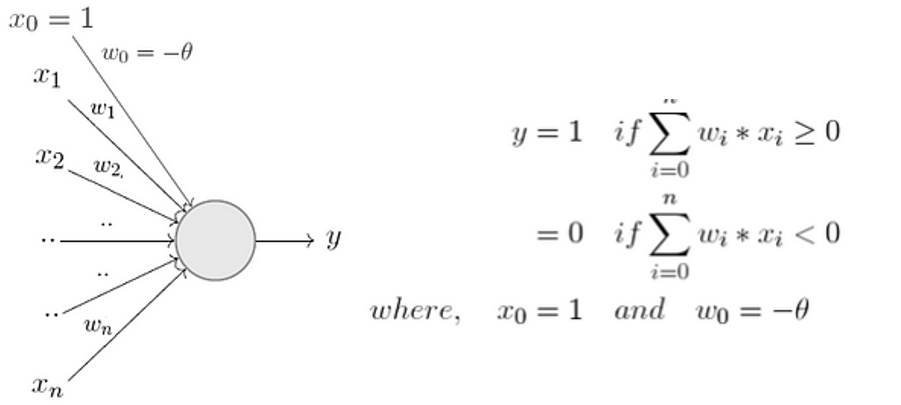
\includegraphics[width=0.7\textwidth]{Chapter1/Figs/1g.png}
\caption[The structure and operation of a perceptron.]{The structure and operation of a perceptron \cite{marvin1969perceptrons}.}
\label{fig:1g}
\end{figure}

\noindent The perceptron, one of the most primitive versions of artificial neural networks, was conceived in the 1940s \cite{mcculloch1943logical} and built in the 1950s \cite{rosenblatt1957perceptron}. It functions as a simple binary classifier, making decisions based on a weighted sum of inputs $x$. During training, the weights $w$ and bias $\theta$ are adjusted to minimize the error on the training set. For instance, a perceptron can be used to distinguish between puppies and kittens based on the intensity of image pixels. \\

\noindent For a period of time, criticisms of the perceptron resulted in reduced funding and research in the field of connectionism \cite{marvin1969perceptrons}. During this time, there was a shift towards rules- and heuristics-based systems \cite{lenat1983eurisko}. However, these methods often lacked robustness and had to be redesigned for individual tasks. In the 1990s, connectionist approaches resurged due to advances in training algorithms, such as backpropagation \cite{rumelhart1986learning}, and the inception of more advanced architectures. \\

\noindent Connectionist approaches resurged in the 1990s, thanks in large part to the improvement of computing devices (Moore's law) and the development of GPUs. The parallelisation of computations, crucial for graphics processing (e.g. in computer games), proved to be useful in statistical machine learning as well, since the same underlying mathematical methods based on linear algebra were used. \\

\noindent After offering solutions for a wide range of AI applications, including but not limited to pattern recognition, natural language processing, modeling and forecasting, voice recognition, bio-informatics, driverless cars, drones, and many more, deep neural networks have attracted increasing attention \cite{hemanth2014performance}. Many changes have been made to various ANN designs in order to improve accuracy and efficiency in diverse applications. \\

\noindent Beginning with Rosenblatt's development of the perceptron in 1958 \cite{hornik1989multilayer}, neural networks have been created by overcoming restrictions such as self-contradiction \cite{hinton2006fast}. A multi-layered feed-forward neural network that can be adequately trained one individual layer at a time and fine-tuned by back-propagation using unsupervised Boltzmann machines (RBMs) was only created in 2006 \cite{sun2014application}. \\ 

\noindent Most modern artificial neural networks include a generalisation of the perceptron known as fully synaptic layers \cite{stone2019artificial}. These layers can have multiple postsynaptic neurons and include a nonlinear activation function $\sigma$. Each synaptic layer consists of pre-synaptic neurons $x$ and post-synaptic neurons $y$, with the synaptic weights stored in a matrix $w$. The activation of each postsynaptic neuron is calculated by taking the dot product of the presynaptic neurons and the corresponding column of the weight matrix (plus bias), followed by the activation function. \\

\noindent To calculate the activation of all postsynaptic neurons, combine them into a vector $y$ and express it as a vector-matrix product of the inputs $x^{\intercal}$ and weights $w$ (plus bias vector), followed by the activation function applied element-wise. Multiple fully connected layers can be combined to form a multilayer perceptron. For example, a multilayer perceptron can be used to recognise handwritten digits \cite{pal2010handwritten}. Whether the network used is a convolutional neural network, a transformer, or some other architecture, fully connected layers are typically included.\\

\noindent However, the use of fully connected layers can be computationally and memory-intensive. In a synaptic layer with $m$ presynaptic neurons and $n$ postsynaptic neurons, the number of weights required is $(m + 1) \times n$, due to the connection of each presynaptic neuron to each postsynaptic neuron, and the presence of one bias weight per postsynaptic neuron. Although computations can be expensive, the majority of the time and energy is spent on transferring data between the memory and compute units of the von Neumann architecture. \\

\noindent Today, neural networks are being emphasised as technology that may be used not only for deep learning challenges, but also in a variety of other AI applications \cite{zbontar2016stereo}. ANNs are a classic example of applications that are restricted by the von Neumann bottleneck. The weights, in the form of large matrices, must be retrieved from memory every time a synaptic layer is utilised. Fetching data from higher-capacity off-chip memory can exacerbate the problem, especially with large artificial neural networks.

\subsection[Machine Learning Goals]{Machine Learning Goals}

During the early stages of artificial intelligence, the majority of work was theoretical. Researchers would create algorithms and rules based on their understanding of the problem to solve it. This soon became clear that for most problems, it was challenging to explicitly write all the necessary rules. For example, traditional computer vision techniques relied on identifying specific hand-defined features in an image. This approach can be effective for tasks such as tracking moving objects, where basic features can be combined with motion principles to monitor an object's movement from one frame to the next. \\

\noindent However, for tasks such as object recognition, it is extremely difficult to define optimal features and rules explicitly. To distinguish between a cat and a dog, or a boat and a truck, one would need to design feature detectors for specific characteristics such as ears, eyes, mouths, and noses. These features would then be used to define rules for different types of objects. This process would require the creation of hundreds of features and rules, each of which would need to be hand-tuned to work properly on the data.  \\

\noindent Machine learning adopts a data-driven approach. Instead of explicitly defining good features and rules, the objective of machine learning is to learn them from the data. The aim is to learn a function that can perform the desired computation on new data points (i.e. different from those used for learning). This is known as generalisation, which enables a machine-learning system to be deployed in the real world. \\

\noindent If the system can only perform well on stimuli it has already encountered, it will always perform poorly on new stimuli unless we can show it every possible stimulus it will ever see (which is impossible for high-dimensional stimuli, such as images). However, if the system can generalize from the training stimuli to similar stimuli, it can perform well on novel stimuli too. The computation desired from a machine learning system is implicitly defined by both the available training data and the learning paradigm. 

\subsection[Learning Archetypes]{Learning Archetypes}

The learning archetype determines the available information for learning and the desired system output. There are three main types: supervised learning, unsupervised learning, and reinforcement learning. These differ in the type of error signal provided to the learner. 

\paragraph{Supervised Learning:} Supervised learning involves learning an input-output mapping using both desired inputs and outputs. It can be divided into regression problems, which have continuous outputs, and classification problems, which have binary outputs representing membership in different categories. The error signal is determined by the difference between the system's output and the desired output.

\paragraph{Unsupervised Learning:} In unsupervised learning, input data (such as images) is used without desired outputs. Instead, the output is implicitly defined based on the input data. Unsupervised learning includes clustering, which groups input data into sets, and dimensionality reduction, which represents data using fewer dimensions than the original representation. The error signal is defined based only on the input. For dimensionality reduction, the goal is to create a system that can represent an input with fewer dimensions while still being able to recreate the input from this representation. The error signal in this case would be the distance between the re-creation and the original input. 

\paragraph{Reinforcement Learning:} Finally, reinforcement learning has a temporal aspect. When given the current state of the environment, the system must choose an action that determines the next state of the environment, which may be probabilistic. The environment rewards certain states, punishes others with negative rewards, and leaves some neutral with no reward. The system aims to achieve maximum total reward over time. \\

\noindent While these are the main categories of learning problems typically studied in machine learning, it is important to note that this is not an exhaustive list. Other paradigms, such as semi-supervised learning, exist where some data points are labelled and others are not, falling between supervised and unsupervised learning. It is worth noting that supervised learning remains the dominant paradigm in object recognition. \\

\noindent As datasets become larger, the cost of fully labelling them increases. Therefore, object recognition is likely to incorporate more semi-supervised and unsupervised methods, and even reinforcement learning. For example, object recognition may be part of a larger problem, such as winning at video games \cite{mnih2013playing}. \\

\noindent In supervised learning, there are two traditional types of problems: regression and classification. The difference lies in the output of the system. Regression systems output one or more continuous values by computing a vector-valued function on the input, whereas classification systems compute a single discrete-valued output that represents the class label of the input. \\

\noindent Recently, there has been growing interest in problems that extend beyond these two categories. An example of a task is predicting multiple labels for an image, such as identifying several objects in an image, or determining verb-like correspondences between objects \cite{karpathy2015deep}. This can also be extended to generating captions for images \cite{xu2015show}, where the model output is a sentence that describes the image.

\subsection[Essential Terminologies]{Essential Terminologies}

Each machine learning system can be described using four components. These components fully characterise the learning problem. If all components are described in detail, anyone should be able to reproduce the result. Machine learning research examines at least one of these components since they determine the capabilities of a learner.

\paragraph{Problem Dataset:} The available data implicitly defines the problem to be learned. In supervised learning, this consists of input/output pairs, while in unsupervised learning, only inputs are used. In reinforcement learning, the data is an environment that specifies the possible states and the rewards associated with each state.

\paragraph{System Architecture:} How the learner is constructed, i.e. what parameters are learned, and how the system output is determined given these parameters and an input value.

\paragraph{Objective function:} In supervised learning, two functions are often used to evaluate a particular set of parameters: one for training and one for testing (evaluation). The training objective function is called a loss function, where zero loss indicates 'perfect' performance, and any positive loss indicates how far we are from perfect performance.

\paragraph{Algorithm Optimization:} The algorithm used to minimize the loss function aims to find the set of parameters that result in the smallest possible loss value, known as the global minimum, on the given dataset within a reasonable amount of time. \\

\noindent To compare different machine learning systems, researchers typically fix the dataset and evaluation objective function, and vary the architecture, loss function, and optimization algorithm. This enables a system to obtain a score on a particular dataset relative to other systems. However, it is important to note that each dataset may only provide a limited view of the capabilities of a particular system, and it is common to test systems on multiple datasets.

\subsection[Fitting and Generalization]{Fitting and Generalization}

In machine learning, there are two main challenges to achieving good generalization to new data: underfitting and overfitting. Underfitting occurs when the system is unable to capture the implicit function being learned, often due to an insufficiently powerful architecture. If a linear network is attempting to learn a nonlinear regression function, no matter how effective our learning methods are, the chosen architecture will not be able to compute the desired function with any set of model parameters. \\

\noindent Another possible reason for this occurrence is when the learning methods cannot identify appropriate parameters for the selected architecture, despite their existence. Recent research has shown that shallow networks can often perform as well as deep networks \cite{ba2014deep}. However, deep networks are still preferred in most cases because it may be difficult or impossible to learn shallow networks directly from the data. This is an example of a situation where the architecture, specifically the shallow network, is theoretically capable of representing the desired function. However, traditional learning methods are ineffective in training it. Instead, it can only be trained by attempting to mimic the deep network. \\

\noindent Overfitting happens when a model learns relationships in the training data that are not useful for the problem at hand. This occurs when the architecture is too powerful for the dataset, causing it to learn idiosyncratic features about specific stimuli instead of general features that apply to new stimuli. An example of extreme memorization is when a learner memorizes every training example and returns the correct answer for all of them during supervised training. However, when presented with new stimuli, the learner outputs random answers, indicating a lack of generalization. To avoid this, it is important to ensure that learners are able to generalize to new examples. \\

\noindent The characteristics of extreme behaviour can manifest in successful learners, where certain parameters in the model may adjust to accommodate idiosyncrasies in specific stimuli. As a result, the model memorises features about these stimuli to identify them, but in a way that does not generalise to other similar stimuli. Overfitting is easy to detect: it occurs when the model performs significantly worse on novel stimuli than on training stimuli. The existence of a generalization error suggests that the model has acquired characteristics from the training set that are not applicable beyond it. \\

\noindent Detecting underfitting can be challenging. One simple measure is to check if the network is achieving zero training error. If not, it may not be able to fully model the desired function and could be underfitting to some degree. However, this assumes that the training data is perfect, with all labels being correct and unambiguous. It also assumes that current architectures are powerful enough to capture all the nuances of the target function, which is often not the case. \\

\noindent Another method of detecting underfitting is to assume that any model that is not overfitting is underfitting. This is a reasonable assumption because there is a narrow range in which a model can perfectly capture a relationship; it is typically either underfitting or overfitting. Moreover, overfitting is not entirely negative; enhancing the training performance on an already overfitting model can still improve the performance on new examples. Overfitting simply indicates that the model is starting to detect false correlations in the training data. Additional training may still assist in identifying some genuine correlations, as well as more false ones. \\

\noindent To address underfitting, either make the architecture more powerful (e.g., increase the number of parameters), or improve the learning methods so that can find better parameter values. Early machine learning often failed even on relatively simple datasets due to the limited computing power that prevented the use of larger models. Convolutional neural networks have been successful because they simplify the learning of parameters. \\

\noindent To address overfitting, the architecture needs to be limited in some way so that it learns more good patterns within the data and fewer spurious ones. Alternatively, the dataset could be expanded so that learning spurious correlations is less advantageous. In some cases, when the model is too large for the dataset, reducing the number of parameters can help. \\

\noindent This is especially effective when incorporating prior knowledge of the problem. However, it is important to note that the number of parameters can only be reduced to a certain extent before the model begins to underfit. At this point, it becomes necessary to limit the parameter values, which is known as regularization. \\

\noindent Simpler forms of regularization place a cost on larger parameter values, preventing the learner from overemphasising certain correlations and relying too heavily on any one feature. Dropout is a form of regularization for neural networks that probabilistically silences neurons, preventing the learner from relying solely on a few features. Finally, expanding the dataset can help to prevent overfitting. This is because the learner is required to perform well on a larger number of training examples, which places more constraints on the parameters. 

\subsection[Benchmark Dataset]{Benchmark Dataset}

The dataset has two main uses: training the system to find the optimal parameter values and testing the system to evaluate the parameter values. The ultimate goal is to determine how well a learner generalizes, or performs when exposed to stimuli it has never encountered before. In supervised learning, datasets are usually divided into separate training and testing subsets. This allows the learner to be exclusively tested on examples it has not seen during training. \\

\noindent Hyperparameters, such as learning rates, model size, and initial parameter values, are not learned but must be chosen a priori. Choosing these parameters without knowledge of the test set is crucial as they can greatly affect the generalization error. Otherwise, hyperparameters may be tuned to the specific test set, resulting in a poor estimator of generalization error as the learner may perform less effectively on examples outside the test set. \\

\noindent To ensure accurate model training, it is common practice to reserve a subset of the data for validation purposes. This subset, known as the validation set, can be used to fine-tune hyperparameters. For instance, a simple approach to finding the optimal learning rate involves testing multiple rates and selecting the one that yields the best performance on the validation set. The resulting model can then be applied to the test set, providing a reliable estimate of generalization error. \\

\noindent Just like the brain has many synapses to solve complex problems, modern machine learning methods have numerous parameters to make them powerful enough to solve real-world problems. To adjust numerous parameters, it is crucial to have datasets that are large enough to encompass a broad range of stimuli that one may encounter in the real world. \\

\noindent For instance, consider all the images that could be captured with a small, low-resolution camera (e.g. 256 x 256 pixels). This encompasses every possible variation of common objects, viewed from any angle and under any lighting condition. Additionally, since each object would only occupy a small portion of the frame, all possible combinations of these objects could be included. The number of potential images is astronomical. \\

\noindent Dataset augmentation is the process of expanding the number of training samples by creating variations on each sample using a core dataset. This can be achieved by including small translations (shifts) of each input, as well as left-right flips. The aim is to increase the diversity of the dataset, which can significantly help reduce the chances of overfitting and better characterize the stimulus space. \\

\noindent Collecting and annotating datasets for supervised learning of object classification is a challenging task. To support the development of new machine learning models and methods, and to facilitate comparison between them, there are several standard datasets publicly available and commonly used in the machine learning community. These datasets are among the most common object classification datasets. \\

\begin{figure}[htbp!] 
\centering    
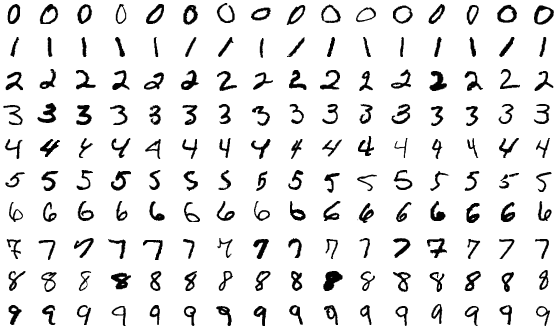
\includegraphics[width=0.7\textwidth]{Chapter1/Figs/1h.png}
\caption[Sample images from MNIST test dataset.]{Sample images from MNIST test dataset \cite{lecun1998gradient}.}
\label{fig:1h}
\end{figure}

\paragraph{MNIST:} This is a collection of handwritten digits taken from US zip codes written on envelopes \cite{lecun1998gradient}. The images have been heavily preprocessed to ensure that each one contains exactly one centred digit in high-contrast greyscale, essentially black and white. Optical character recognition of handwritten digits is a challenging task. The first successful attempt at this problem marked a turning point in machine learning. Although the dataset is no longer considered challenging for state-of-the-art methods, it is still commonly used as a benchmark for new models and methods due to its relatively small size. This allows for efficient training even with slower methods such as online learning and spike-based methods. 

\paragraph{SVHN:} This dataset is comprised of digits extracted from Google Street View images of house numbers \cite{netzer2011reading}. The styles of digits, as well as the backgrounds, lighting, colours, and contrast, exhibit significant variation. The images have been preprocessed to center on the target digit for classification, but they may also contain whole or partial distractor digits to the sides. To ensure clarity, technical term abbreviations will be explained when first used. This dataset is considerably more challenging than MNIST, but still relatively easy compared to datasets composed of objects. 

\paragraph{CIFAR:} The CIFAR-10 and CIFAR-100 datasets comprise small images (32 × 32 pixels) from 10 or 100 categories, respectively \cite{krizhevsky2009learning}. All images in this dataset are in full colour and were taken from the Tiny Images Dataset \cite{torralba200880}. Although the dataset is the same size as the SVHN dataset, it is considerably more challenging. Human performance on CIFAR-10 has been estimated to be 94\% accurate \cite{karpathy2011lessons}. CIFAR-100 is even more challenging due to the increased diversity of object categories. Each category encompasses a wide range of visual features and has a larger variety of object poses. For instance, CIFAR-10 includes a category named 'dog', which comprises images of various dog breeds captured from different angles and with diverse appearances. CIFAR-100 poses an additional challenge as it contains more categories, making it less likely to guess the correct one by chance. Furthermore, many of the categories are similar, such as 'shrew' and 'mouse', and it is challenging to distinguish between them consistently using small images taken from various angles.

\paragraph{ImageNet:} The ILSVRC-2012 dataset, also referred to as the ImageNet dataset, comprises images from the ImageNet database \cite{russakovsky2015imagenet}. It was utilised for the 2012 ImageNet Large Scale Visual Recognition Challenge. The ImageNet database consists of medium to high resolution images that are organised into hierarchical categories called synsets (short for 'synonym set'). It contains millions of annotated images. The ILSVRC-2012 dataset is a subset of images used for the 2012 ImageNet Large Scale Visual Recognition Challenge competition. It contains images tagged with 1000 different categories, mainly consisting of animal species, plants, household objects, vehicles, and building/room types (both exterior and interior). The images vary in size, and pre-processing often involves scaling and cropping them to 256 × 256 pixels. This dataset is more challenging than the previous ones due to the increased number of categories and the presence of multiple objects in the images. It can be ambiguous to determine the primary object of focus in some cases. \\

\noindent Modern machine learning algorithms have performed well in addressing these challenges. Many algorithms have published both top-5 and top-1 results, where top-5 indicates that the image is considered correctly classified if the actual label for the test image is in any of the top five categories predicted by the algorithm. Similarly, top-1 means that the top prediction must match the correct label. Top-5 classification is useful for handling ambiguous images with multiple featured objects and for distinguishing between similar categories that may be difficult to differentiate from all angles, such as certain breeds of dogs.

\subsection[Network Architectures]{Network Architectures}

The two primary building elements of fully linked artificial neural networks (ANNs) are synapses and neurons. The neurons add up the incoming scaled signals and then convert the sum, while the synapses scale the signals. Neural networks nowadays consist of multilayer perceptrons (MLPs), convolutional neural networks (CNNs), and recurrent neural networks (RNNs), as Figure \ref{fig:1i} illustrates.

\begin{figure}[htbp!] 
\centering    
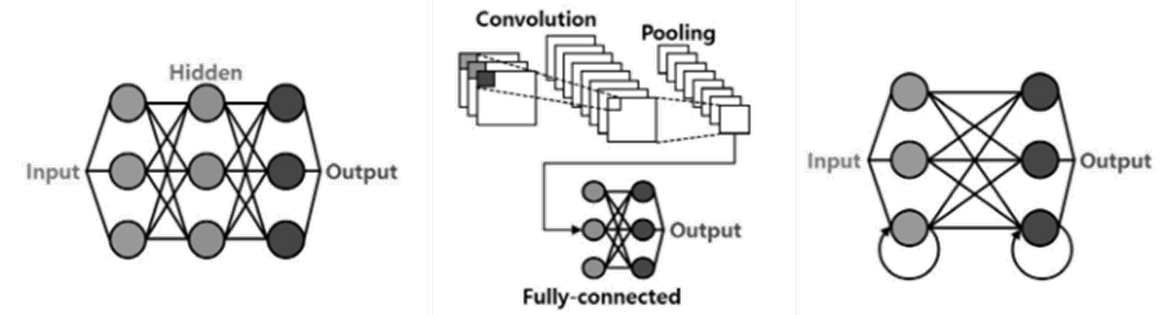
\includegraphics[width=1\textwidth]{Chapter1/Figs/1i.png}
\caption[The backbone architectures of neural networks]{The backbone architectures of neural networks, left to right: multilayer perceptron (MLP), convolutional neural networks (CNN), and recurrent neural networks (RNN) \cite{stone2019artificial}.}
\label{fig:1i}
\end{figure}

\noindent Neurons are shown as circles in the picture, and the connections between those neurons are represented as synapses, also known as weights. The signal travels to the right until it reaches the output layer after inputs are provided to a neural layer known as the input layer. There are usually several hidden layers between the input and output layers. In addition, bias neurons are often present in both the input layer and the hidden layers. Lastly, synaptic layers are the collections of synapses that connect two nearby neural layers. \\

\noindent More formally, MLPs are back-propagation-trained basic feedforward deep neural networks having an input layer, one or more hidden layers, and an output layer \cite{pelaez2014ischemia}. For MLPs with 3–10 neuron layers, straightforward classification tasks like handwriting pattern recognition are straightforward application cases.  Color pictures, which are composed of three 2D drawings with changing pixel intensities in the three recognised colour channels of red, green, and blue, are one type of data that CNNs are designed to function with \cite{matsugu2003subject}. \\

\noindent Some of the inherent characteristics of these signals that CNNs may employ include connectivity, weight sharing, pooling, and the use of many layers. This led to CNNs making a number of useful advancements and seeing extensive application in the field of computer vision \cite{ji20123d}. Typically, 5-100 layer CNN architectures are used for visual processing tasks like facial recognition and image segmentation \cite{szegedy2017inception}. \\

\noindent RNNs are constructed as networks of neurons with these extra connections, based on the same notion as neural networks with additional feedback loops \cite{funahashi1993approximation}. The availability of these additional feedback loops contributes to RNNs' capacity to retain information while processing incoming inputs \cite{lukovsevivcius2009reservoir}. This architecture is suitable for tasks that need processing data while taking into account older inputs, such historical data, but still dealing with present input \cite{mikolov2011extensions}. \\

\noindent This architecture allows for the training of many behaviours, including those involved in sequential processing tasks, that are not conducive to learning using conventional neural networking learning techniques \cite{zhang2005design}. RNNs have therefore been used in many data processing applications, such as voice recognition, translations, and natural-language processing \cite{hardy2018encoding}. \\

\noindent In summary, dramatic developments in neural network technology have resulted in several computer breakthroughs that are both more energy efficient and inspired by the human brain \cite{maass1997networks}. These modifications affect not just software but also physical computer architecture and hardware \cite{goodman2008brian}. New kinds of devices with far superior qualities to traditional memory devices are being investigated extensively \cite{nageswaran2009configurable}, with memristor devices being regarded as neuromorphic device options for neural networks \cite{kasabov2014neucube}. Memristor devices have been shown to offer favourable characteristics for various architectures \cite{querlioz2013immunity}.

\subsection[Matrix-Vector Multiplication]{Matrix-Vector Multiplication}

A weighted bipartite graph is formed by each synaptic layer and the two neuronal layers that encircle it. The nodes in the two neuronal layers are the neurons, and the edges are the synapses in the synaptic layer. A vector matrix product can be used to summarise the summation function of neurons and the scaling function of synapses, $\textbf{y} := \textbf{xW}$. Here, \textbf{W} is a weight matrix, \textbf{y} is a vector holding the synaptic layer's outputs, and \textbf{x} is a vector holding the inputs to the synaptic layer. \\

\noindent As was previously established for perceptron, bias neurons, which typically have a constant input of 1, are found in presynaptic layers. The bias neuron's weights may be expressed as a vector since an input of 1 is applied. This modified the equation to $\textbf{y} := \textbf{xW} + \textbf{b}$, where \textbf{b} is a vector that represents the bias neuron's associated synaptic strengths. On the other hand, the bias weights may be added to the weights matrix \textbf{W}, and the input of 1 can be merged with the remaining inputs, \textbf{x}, for each given layer. This will often be done implicitly and resulted in the form below (\ref{eq:1.1}).
\\

\begin{align}
\begin{matrix}
& \textbf{W} & \\
& \begin{bmatrix}
    w_{1,1} & w_{1,2} & \cdots & w_{1, m} \\
    w_{2,1} & w_{2,2} & \cdots & w_{2, m} \\
    \vdots & \vdots & \vdots & \vdots \\
    w_{n, 1} & w_{n, 2} & \cdots & w_{n, m}
\end{bmatrix} &\\
\end{matrix}
\begin{matrix}
  & \textbf{x} & \\
 & \begin{bmatrix}
x_{1} \\
x_{2} \\
\vdots \\
x_{n}
\end{bmatrix} &\\
\end{matrix}
\begin{matrix}
 & = & \\
\\
\\
&=&  \\
\\
\end{matrix}
\begin{matrix}
  & \textbf{y} & \\
 & \begin{bmatrix}
y_{1} \\
y_{2} \\
\vdots \\
y_{m}
\end{bmatrix} &\\
\end{matrix}
\label{eq:1.1}
\end{align}

\noindent As mentioned before, the postsynaptic neurons usually change the signals in addition to summing. Applying an activation function does this. The $(i + 1)^{th}$ synaptic layer's inputs can be stated as follows:
\begin{align}
    x_{i+1} = \sigma_i\left( x_i W_i + b_i \right) \label{eq:1.2}
\end{align}

\noindent The notation $x_{i+1}$ and $x_i$ represents the inputs to the $(i + 1)^{th}$ and $i^{th}$ synaptic layers, respectively. The weight matrix of the $i^{th}$ synaptic layer, $W_i$, is represented by the vector $b_i$, which is a vector of weights connected to the bias neuron in the presynaptic neuronal layer of the $i^{th}$ synaptic layer. The vector-valued activation function associated with the postsynaptic neuronal layer of the $i^{th}$ synaptic layer is represented by $\sigma_i$. Assuming that there are two fully connected layers ANN, the output is as follows:
\begin{align}
    y = \sigma_2 (x_2 W_2 + b_2) = \sigma_2 (\sigma_1(x_1 W_1 + b_1) W_2 + b_2) \label{eq:1.3}
\end{align}

\noindent By adding nonlinearities, activation functions are utilised to expand network capacity \cite{pomerat2019neural}. The logistic function (\ref{eq:1.4}), the hyperbolic tangent (\ref{eq:1.5}), the rectified linear unit (ReLU) (\ref{eq:1.6}), and the leaky ReLU (\ref{eq:1.7}) are the most often used options for activation functions \cite{zhang2018efficient}; corresponding scalar formulas for these functions are provided below:

\begin{align}
    g\left ( z \right ) &= \frac{1}{1 + e^{-z}} \label{eq:1.4} \\
    g\left ( z \right ) &= \frac{e^z - e^{-z}}{e^z + e^{-z}} \label{eq:1.5} \\
    g\left ( z \right ) &= max\left \{ 0, z \right \} \label{eq:1.6} \\
    g\left ( z \right ) &= max\left \{ \epsilon z, z \right \} \label{eq:1.7} 
\end{align}

\noindent The existence of an activation function in an ANN determines the requirement for several hidden layers. This is due to the fact that a single linear transformation may be written as a sequence of linear transformations, which are represented as linear products. Take an ANN with two synaptic layers as an example. If no activation functions were used, its outputs may be represented as a single vector-matrix product with bias added. \\

\begin{figure}[htbp!] 
\centering    
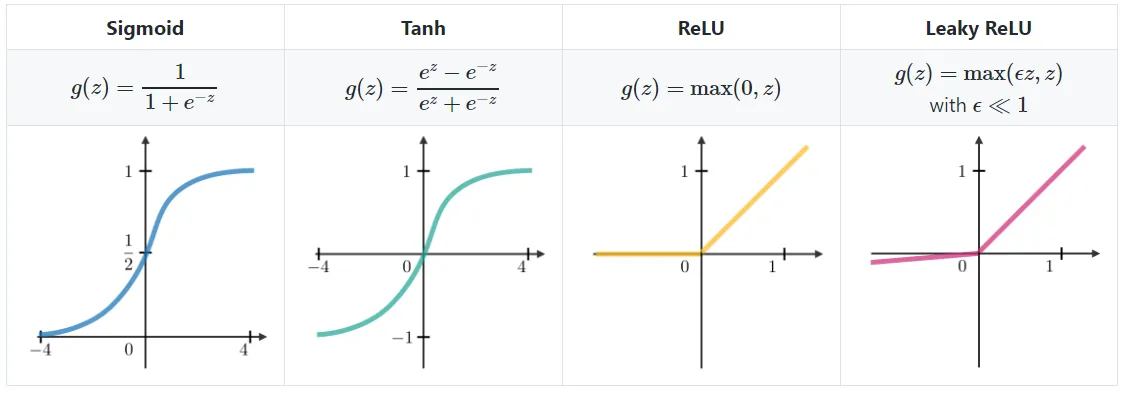
\includegraphics[width=1\textwidth]{Chapter1/Figs/1j.png}
\caption[Activation functions commonly used in ANN]{Activation functions commonly used in ANN with the expressions labelled.}
\label{fig:1j}
\end{figure}

\noindent The network's capacity is increased by non-linear activation functions, which stop several weight matrices (and bias vectors) from "collapsing" into one. Furthermore, if the network is big enough, an ANN with non-polynomial activation functions may accurately estimate any continuous function to any degree \cite{leshno1993multilayer}. Neural networks may therefore be used to fit data of unlimited complexity.

\subsection[Training and Inference]{Training and Inference}

ANNs are often used for applications like regression and classification. To illustrate, a neural network may be used to classify photographs of handwritten digits. The picture's pixels are translated into a vector $\textbf{x}$, which is then fed into the ANN, which generates a vector $\textbf{y}$ with ten elements, each representing the likelihood that the image represents a certain digit. \\

\noindent In general, this process is known as inference, and it involves determining a class (or a specific value in the case of regression) based on the inputs $\textbf{X}$. The outputs of ANN (or any other supervised learning model) utilised in inference may be stated as $\textbf{Y} = f(\textbf{X, W})$. In the context of artificial neural networks (ANNs), the model parameters, represented by $\textbf{W}$, represent synaptic weights. The recursive formula of equation (\ref{eq:1.2}) may be used to fully connected ANNs with $n$ synaptic layers to achieve the specified form. \\

\noindent A supervised learning model's parameters $\textbf{W}$ are determined via a process known as training \cite{bishop2006pattern}. The goal of this procedure is to match certain training input data $\textbf{X}_{train} $ to training target data $\textbf{T}_{train}$. Once a model has been trained, its outputs $\textbf{Y}$ should be able to predict test targets $\textbf{T}_{test}$ from a set of test inputs $\textbf{X}_{test}$. Training usually requires specifying a loss function, which defines the closeness of the outputs to the target data and then seeks to reduce it. The squared-error (\ref{eq:1.8}) and cross-entropy (\ref{eq:1.9}) loss functions are two of the most commonly used \cite{kline2005revisiting}. 
\begin{align}
    E\left ( \mathbf{W} \right ) &= \frac{1}{M} \sum_{m=1}^{M} \sum_{p=1}^{P} \left ( \left [ \mathbf{f} \left ( \mathbf{X}_{m,*}, \mathbf{W} \right ) \right ]_{p} - \mathbf{T}_{m,p} \right )^{2} \label{eq:1.8} \\
    E\left ( \mathbf{W} \right ) &= \frac{1}{M} \sum_{m=1}^{M} \sum_{p=1}^{P}  \mathbf{T}_{m,p} ln \left ( \left [ \mathbf{f} \left ( \mathbf{X}_{m,*}, \mathbf{W} \right ) \right ]_{p}\right ) \label{eq:1.9}
\end{align}

\noindent The feed-forward inference function, represented by $\mathbf{f}$, accepts input data from the matrix $\mathbf{X} \in \mathbb{R}^{M \times N}$ , where $\mathbf{M}$ is the number of instances, $\mathbf{N}$ is the number of inputs, and $\mathbf{P}$ is the number of classes. Performance of the function $\mathbf{f}$ is evaluated using target data $\mathbf{T} \in \mathbb{R}^{M \times P}$. In supervised learning, the network's objective or loss function determines the quantity to optimize, linking the actual outputs to the desired outputs. It is commonly referred to as a cost or loss that we aim to minimize. This cost reflects how poorly the network performs on the training dataset. \\

\noindent A crucial differentiation exists between loss functions and error functions. In regression problems, these functions are often identical, but in classification problems, they differ. An error function measures the amount of error a network produces. In classification, this is usually the number of incorrectly classified examples divided by the total number of examples. A sample is deemed incorrectly classified if the output with the highest value is not the correct output. \\

\noindent The loss function for classification is dependent on the output values. For instance, the function may impose a penalty (i.e. non-zero loss) on an example if the network output for the correct class is not as high as intended, or if the margin between the correct output and the next most active output is not as large as intended. This implies that even correctly classified examples may still have a non-zero loss.\\

\noindent Overall, this pushes the classifier to not only get the answer right, but to get it right by a significant margin, ideally making the classifier more robust and better able to generalise to new inputs. The loss function is also continuous and differentiable, whereas the error function can be discrete; this makes the loss function easier to optimise, as the derivative(s) can be used in the optimisation.

\subsection[Backpropagation Algorithm]{Backpropagation Algorithm}

The backpropagation (BP) algorithm, also known as 'backwards propagation of gradients' or 'backprop', is the algorithm responsible for the recent success of machines in object recognition tasks. Although the algorithm was introduced in the 1980s \cite{rumelhart1986learning}, it was only mildly successful at the time due to a lack of computational resources. As computers developed and machine learning became better understood, backpropagation became increasingly useful. This culminated in LeNet \cite{lecun1998gradient}, a deep convolutional network that marked the first significant success on the MNIST handwritten digit dataset and a seminal success of neural networks in general. \\ 

\noindent Since then, the algorithm has gained popularity. In the 2000s, backpropagation was used to fine-tune various types of deep networks. It was applied at the end of the training algorithm to make moderate adjustments to network weights, resulting in a significant decrease in error at the end of the training regime. Other algorithms were used for pretraining, which involved determining initial weights that could be moderately successful at a task and provide a starting point for backpropagation. \\

\noindent Layer-wise pretraining is a method in which each layer of a deep network is trained as an autoencoder or restricted Boltzmann machine (RBM) to represent the information in the previous layer. This unsupervised training initializes the network to a state where the final hidden layer retains a significant amount of input information. Backpropagation can then be used to train the output classifier and fine-tune the weights of the previous layers. \\

\noindent Backpropagation has just recently—roughly since 2010—been utilised to train networks from start. This is made feasible by the convergence of three key components. It was possible to train larger models on larger datasets in an acceptable period of time by increasing computing power, particularly with GPUs. Rectified linear units (ReLUs), which are scale-invariant and reduce the likelihood of vanishing and inflating gradient issues, making training less sensitive to the initial weights. When paired with these techniques, convolutional networks—which had been effectively applied a decade earlier—markedly reduced the number of parameters when compared to fully linked techniques like RBMs. \\

\noindent Presently, nearly all deep networks are trained using backpropagation as the primary workhorse. Backpropagation is a technique used to calculate the gradients of the network parameters in relation to an objective function. It solves the spatial credit assignment problem, which involves identifying the hidden units responsible for a particular error at the network output and determining which parameters should be adjusted to reduce the error most efficiently. In other words, it assigns credit or blame to the hidden units for their contribution to the network output. This was a significant challenge for early neural network researchers.

\subsection[Stochastic Gradient Descent]{Stochastic Gradient Descent}

Backpropagation offers a method for obtaining the first-order derivative (gradient) of the cost function concerning the network parameters. However, it does not specify how to utilize this gradient to minimize the cost. There are several potential methods to achieve this. The simplest approach involves adjusting the parameters in the direction of the negative gradient. The gradient indicates the direction in which the cost increases most rapidly. To decrease the cost quickly, it is moved in the direction of the negative gradient. This process is known as gradient descent. \\

\noindent Given the complexity of ANNs and data, it is impossible to analytically calculate the set of weights W that minimises $E(\mathbf{W})$. Gradient descent is typically used for this type of minimization. At time step $\tau$, the gradient $\triangledown_i E$ of the loss function with respect to weights in the $i^{th}$ synaptic layer is determined. Weights are then gently changed in the opposite direction of the gradient. This technique is done recursively several times and may be formalised using the recursive formula (\ref{eq:1.10}), where $\eta \in \mathbb{R}_{>0}$.
\begin{align}
    \mathbf{W}_{i}^{\tau + 1} = \mathbf{W}_{i}^{\tau} - \eta \triangledown_i E \left ( \mathbf{W}^{\tau} \right ) \label{eq:1.10}
\end{align}

\noindent By definition, taking only a very small step in this direction will decrease the cost, as the function may only decrease for a very short distance before starting to increase again. However, in practice, we must take a significant step in the gradient direction. The step size is modulated by the learning rate, which is multiplied by the gradient to determine the step. There is a trade-off between a large and small learning rate. A large learning rate allows for quicker convergence on smooth, well-conditioned objectives, while a small learning rate ensures stability and convergence on more ill-conditioned problems. As long as the learning rate is sufficiently small, gradient descent can converge for any problem. \\

\noindent During gradient descent, the gradient is computed across all training samples (known as the batch) for each parameter update, which can be computationally expensive. Stochastic gradient descent (SGD) addresses this issue by using only a portion of the training set to estimate the gradient at each iteration, with the understanding that this may occasionally increase the overall cost. At each iteration, a noisy or stochastic estimate of the gradient is computed. If the corresponding parameter updates are beneficial on average, the overall cost should decrease. The mini-batch is the set of examples used to estimate the gradient. \\

\noindent The mini-batch size is a crucial parameter in SGD. A larger mini-batch provides a more accurate gradient estimate, but also requires more computation per mini-batch. Therefore, selecting the mini-batch size involves balancing these two criteria. In practice, mini-batches usually contain 20 to 100 examples. SGD is a widely used method due to its simplicity and effectiveness on various problems. \\

\noindent Most neural networks are too large and complex for second-order methods, which require the explicit computation of second-order derivatives (known as the Hessian) and are therefore not feasible. Even methods that estimate the second-order derivatives, such as L-BFGS, cannot handle the size of modern neural networks, as the number of elements in the Hessian is equal to the number of possible pairs of parameters in the model \cite{liu1989limited}. Hessian-free optimization can avoid the vanishing and exploding gradient problems that are particularly potent in recurrent neural networks \cite{martens2010deep}, making it a popular choice for improving their performance.

\subsection[Gradients Initialization]{Gradients Initialization}

During artificial neural network (ANN) optimization, two common issues arise: the vanishing and exploding gradient problems. These problems become more prevalent as networks become deeper or recurrent, as recurrent networks are often optimized like deep networks with tied parameters between layers. The vanishing gradient problem occurs when the gradient's magnitude approaches zero, causing the optimization process to slow down significantly. \\

\noindent A saddle-point in the parameter space is indicated, which is a common issue when optimizing ANNs \cite{dauphin2014identifying}. If the gradient of one layer approaches zero prematurely, such as when most neurons in a layer become inactive, then the gradients for other layers will also quickly approach zero. This is because the cost can only be reduced to a certain extent when one layer is not functioning. \\

\noindent The problem of exploding gradients arises when the gradients become too large too quickly. This is usually due to instability in the SGD algorithm caused by a learning rate that is too high. Once the algorithm becomes even slightly unstable, it is difficult for it to regain stability. For instance, a high learning rate can cause the algorithm to overshoot the minimum in the gradient direction and end up in an area of higher cost. This higher cost leads to the next gradient, and consequently the next step, being too large, resulting in an even higher cost. As a result, the algorithm spirals out of control. \\

\noindent The vanishing and exploding gradient problems may arise from improper network initialization. Layers with excessively large or small parameters can cause issues, particularly when using sigmoid nonlinearities, which have zero derivatives for both large negative and positive values. Several initialization schemes have been developed to mitigate these problems. Several initialization schemes have been developed to mitigate these problems. The concept underlying these methods is that the variance information transmitted both forwards (activations) and backwards (derivatives) through the network should remain constant. 


\section[Thesis Outline]{Thesis Outline}

